\documentclass{article}

\usepackage[utf8]{inputenc}
\usepackage[T1]{fontenc}
\usepackage[english,norsk]{babel}   %Engelsk først så norsk, så norsk blir prioritert
\usepackage{graphicx}
\usepackage{amsmath}        %For å kunne skrive matte
\usepackage{listings}       %For å kunne skrive inn kode med fin formatering
\usepackage{multicol}       %Importerer pakken for multikolonner til teksten
\usepackage[margin=2.54cm]{geometry}    %Definerer hva bredden til teksten er
\usepackage{wrapfig}    %Importerer pakken for å ha bildene i teksten
\usepackage[font = small]{caption}
\usepackage{textcomp}
\usepackage{mathrsfs}   %For å få fancy E til bildene

\usepackage{amssymb} %Fra Erlend for å bruke hakemerke?? Vet egt. ikke

%Definerer hyperlinker og dens farger
\usepackage{hyperref}
\hypersetup{
    colorlinks,
    citecolor=blue,
    filecolor=black,
    linkcolor=blue,
    urlcolor=blue
}

%-----------------------------------
\iffalse
%Definerer farger til kodeeksemplene i PDF-en
\usepackage{color}

\definecolor{codegreen}{rgb}{0,0.6,0}
\definecolor{codegray}{rgb}{0.5,0.5,0.5}
\definecolor{codepurple}{rgb}{0.58,0,0.82}
\definecolor{backcolour}{rgb}{0.95,0.95,0.92}

\lstdefinestyle{mystyle}{
    backgroundcolor=\color{backcolour},
    commentstyle=\color{codegreen},
    keywordstyle=\color{magenta},
    numberstyle=\tiny\color{codegray},
    stringstyle=\color{codepurple},
    basicstyle=\footnotesize,
    breakatwhitespace=false,
    breaklines=true,
    captionpos=b,
    keepspaces=true,
    numbers=left,
    numbersep=5pt,
    showspaces=false,
    showstringspaces=false,
    showtabs=false,
    tabsize=2
}

\lstset{style=mystyle}
\fi


%--------------------------------------

\setlength{\parindent}{0pt} %Ingen indent automatisk for nye linjer
%\setlength{\columnsep}{2mm} %Column separation - til multicolumn

%\setlength{\arrayrulewidth}{1mm}   %Hvilken tykkelse tabellene skal ha
\setlength{\tabcolsep}{2mm}     %Lengden mellom hver kolonne
\renewcommand{\arraystretch}{1.5}   %Hvor stor avstand det skal være mellom radene

\iffalse    %midlertidig endre bredden på teksten
If you want to change this temporarily, you can write:
\savegeometry{mydefaultgeometry}
\newgeometry{margin=3in}
And then later you can call:
\loadgeometry{mydefaultgeometry}
\fi

%for å fjerne overskriften "refrences" som kommer automatisk når man bruker bibtex
\usepackage{etoolbox}
\patchcmd{\thebibliography}{\section*{\refname}}{}{}{}

%lage exercises på norsk, slik at det står oppgave. også definere dette som en ny kommando
\newcounter{excount}
\newenvironment{exercise}[1][]{\addtocounter{excount}{1} \noindent {\bf Oppgave
\arabic{excount} \ \ #1}\hspace{2mm}}{\vspace{4mm}}


%----------------------

\usepackage{float}
%\restylefloat{table}

%----------------------

\usepackage{tikz}
\usetikzlibrary{patterns}

\usetikzlibrary{shapes.misc}
% From http://tex.stackexchange.com/questions/123760/draw-crosses-in-tikz
\tikzset{cross/.style={cross out, draw=black, fill=none, minimum size=2*(#1-\pgflinewidth), inner sep=0pt, outer sep=0pt}, cross/.default={3pt}}

\usetikzlibrary{decorations.markings}

%------------------

%dette brukes med \begin{python}
\usepackage{pythonhighlight}

\lstdefinestyle{mystyle}{
    numbers=left,
    numbersep=5pt,
}

\lstset{style=mystyle}


%-----------------------

%figurtekst under, tabelltekst over

%LEGGE TIL STJERNER VED SECTION FJERNER NUMMERERINGEN!!!!!!!!!!!!!!!!!!!!!!!!!!!!!!!!
%men da syntes ikke avsnittene i innholdsfortegnelsen!!!!!!!!!!!!!!!!!!!!!!!!!!!!!!!!

%------------------------------------------------------------------------------

\begin{document}

\addtocounter{page}{0}

\title{Project A20 \\
      \large FYS-MENA4111}
\date{\today \\
    \vspace{1mm}
    \large Week 44-}

\author{Erlend Tiberg North \& Alexandra Jahr Kolstad}

\maketitle


%\newpage

%--------------- Her starter skrivingen ---------------------------------------

%\begin{multicols}{2}


%---------------------- Abstract -----------------------------------------
\vspace{1cm}


\begin{center}

{\Large\textbf{Abstract}} \label{sec:Abstract} \\

    \vspace{1cm}

\end{center}


\newpage

%-------------------- Table of contents -----------------------------------
\vspace{1cm}

\tableofcontents

\vspace{1cm}

%---------------------------------------------------------------------------------

\textbf{Ting å gjøre:}
\begin{itemize}
    \item lage en mappe på saga for begge
    \subitem \textbf{done}
    \item skaffe POSCAR, jobfile og INCAR (de andre følger fra disse)
    \subitem \textbf{done}
    \item sjekke at den konvergerer (decent ENCUT og KPOINTS)
    \subitem \textbf{done}
    \subitem The data shows that we should use 450eV for ENCUT as that is the 1st job with a difference less than 3meV.
    \subitem For k-density we see that even the lowest value, 1.0, is within 3 meV (1.0 gives around 1.75 meV), so this can be used. However, the data shows that 3.0 is below 1 meV, with 4.0 being identical in energy to 5.0. This can possibly be discussed in group, but 1.0 should technically be enough for k-density.
    \item relaxe POSCAR og static etter relax POSCAR
    \subitem \textbf{done}
    \item total og relativ energi (fra static etter relax)
    \subitem \textbf{done}
    \item DOS (båndgap) og LDOS (båndstruktur)
    \subitem \textbf{done}
    \item romlig elektronstruktur; 3D-plot av ladningstetthet (VESTA)
    \item bytte ut hydrogen i alkoholgruppen med lantanoidatomer (Yb, Nd, Tm og Y)
    \item relaxe POSCAR og static etter relax POSCAR
    \item total og relativ energi (fra static etter relax)
    \item DOS (båndgap) og LDOS (båndstruktur)
    \item romlig elektronstruktur; 3D-plot av ladningstetthet (VESTA)
\end{itemize}

\vspace{1cm}

\textbf{Ting å ha i \LaTeX:}
\begin{itemize}
    \item abstrakt
    \item kort introduksjon av materialet
    \item kort om metode, valg av paramtere (CUTOFF, etc)
    \item presentasjon av de viktigste resultatene
    \item diskusjon av hvordan resultatene kan tolkes, f.eks. sammenligne til eksperimenter eller tidligere beregninger i litteraturen
    \item konklusjon/oppsummering
    \item kilder
    \item appendix ?
\end{itemize}

\vspace{1cm}

\textbf{\large{OBS: husk å lagre bilder for rapporten og presentasjonen mens man gjør beregningene}}

\section{Introduction}  \label{sec:Introduction}

\vspace{1cm}

\section{Method}    \label{sec:Method}

  \subsection{Energy convergence}

    ENCUT: 300 to 900

  \subsection{K-points convergence}

    K-point density: 1.0 to 6.0

\vspace{1cm}

\section{Results}   \label{sec:Results}

  \subsection{Energy convergence}

    Started to convergence around 450 eV for ENCUT.

  \subsection{K-points convergence}






\vspace{1cm}

\section{Discussion}    \label{sec:Discussion}

\vspace{1cm}

\section{Conclusion}    \label{sec:Conclusion}


%--------------------- References --------------------------------------------
\vspace{1cm}

\section{References} \label{sec:References}

    \begin{thebibliography}{}

    \bibitem{laereboken}
    Ben G. Streetman \& Sanjay Kumar Banerjee, 2016, \textit{Solid State Elctronic Devices seventh edition}, Pearson Education


    \end{thebibliography}


%------------------ Appendix ------------------------------------

\appendix

\section{Convergence energy}

  \begin{figure}[H]
      \centering
      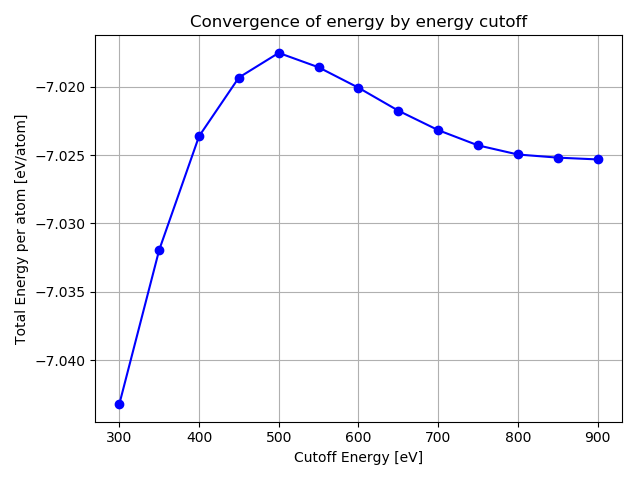
\includegraphics[width = 11cm]{../fig/convergence_energy.png}
      \caption{. }
      \label{fig:convergence_energy.png}
  \end{figure}

  \begin{figure}[H]
      \centering
      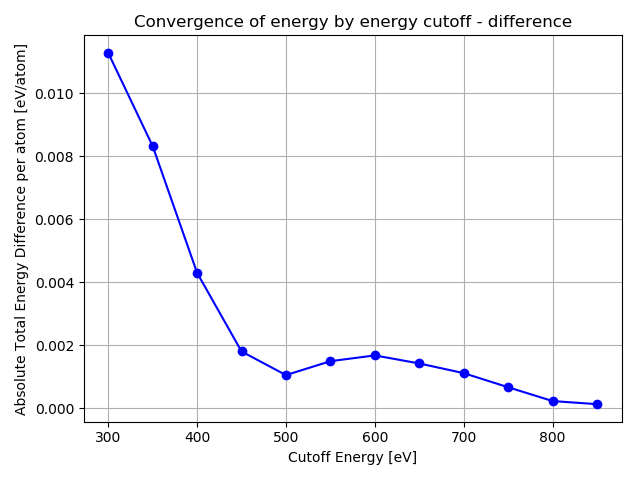
\includegraphics[width = 11cm]{../fig/convergence_energy_difference.png}
      \caption{. }
      \label{fig:convergence_energy_difference.png}
  \end{figure}

\vspace{1cm}

\section{Convergence kpoints}

  \begin{figure}[H]
      \centering
      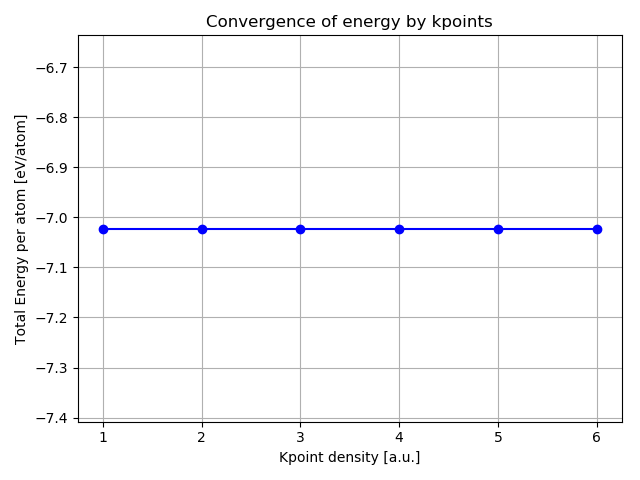
\includegraphics[width = 11cm]{../fig/convergence_kpoints.png}
      \caption{. }
      \label{fig:convergence_kpoints.png}
  \end{figure}

  \begin{figure}[H]
      \centering
      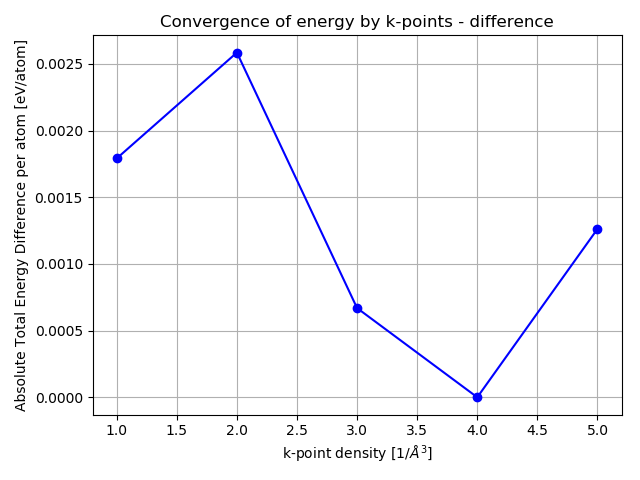
\includegraphics[width = 11cm]{../fig/convergence_kpoints_difference.png}
      \caption{. }
      \label{fig:convergence_kpoints_difference.png}
  \end{figure}

\vspace{1cm}

\section{DOS-bilder}


  \iffalse
  \begin{figure}[H]
      \centering
      \includegraphics[width = 11cm]{../fig/DOS_staticbefore_CONTCAR.png}
      \caption{. }
      \label{fig:DOS_staticbefore_CONTCAR}
  \end{figure}

  \begin{figure}[H]
      \centering
      \includegraphics[width = 11cm]{../fig/DOS_staticbefore_CHGCAR.png}
      \caption{. }
      \label{fig:DOS_staticbefore_CHGCAR}
  \end{figure}

  \begin{figure}[H]
      \centering
      \includegraphics[width = 11cm]{../fig/DOS_relax_CONTCAR.png}
      \caption{. }
      \label{fig:DOS_relax_CONTCAR}
  \end{figure}

  \begin{figure}[H]
      \centering
      \includegraphics[width = 11cm]{../fig/DOS_relax_CHGCAR.png}
      \caption{. }
      \label{fig:DOS_relax_CHGCAR}
  \end{figure}

  \begin{figure}[H]
      \centering
      \includegraphics[width = 11cm]{../fig/DOS_staticafter_CONTCAR.png}
      \caption{. }
      \label{fig:DOS_staticafter_CONTCAR}
  \end{figure}

  \begin{figure}[H]
      \centering
      \includegraphics[width = 11cm]{../fig/DOS_staticafter_CHGCAR.png}
      \caption{. }
      \label{fig:DOS_staticafter_CHGCAR}
  \end{figure}
  \fi


  \begin{figure}[H]
      \centering
      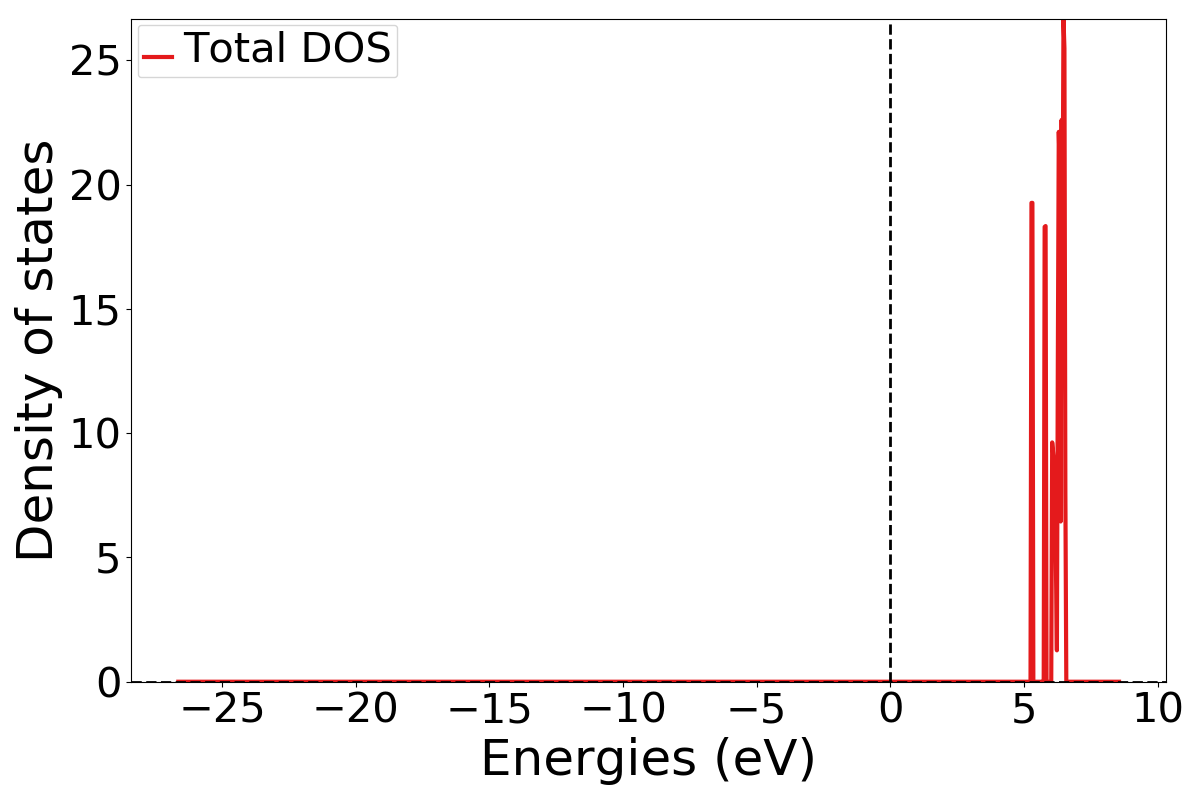
\includegraphics[width = 11cm]{../fig/DOS_k4_TDOS_1.png}
      \caption{. }
      \label{fig:DOS_k4_TDOS_1}
  \end{figure}

  \begin{figure}[H]
      \centering
      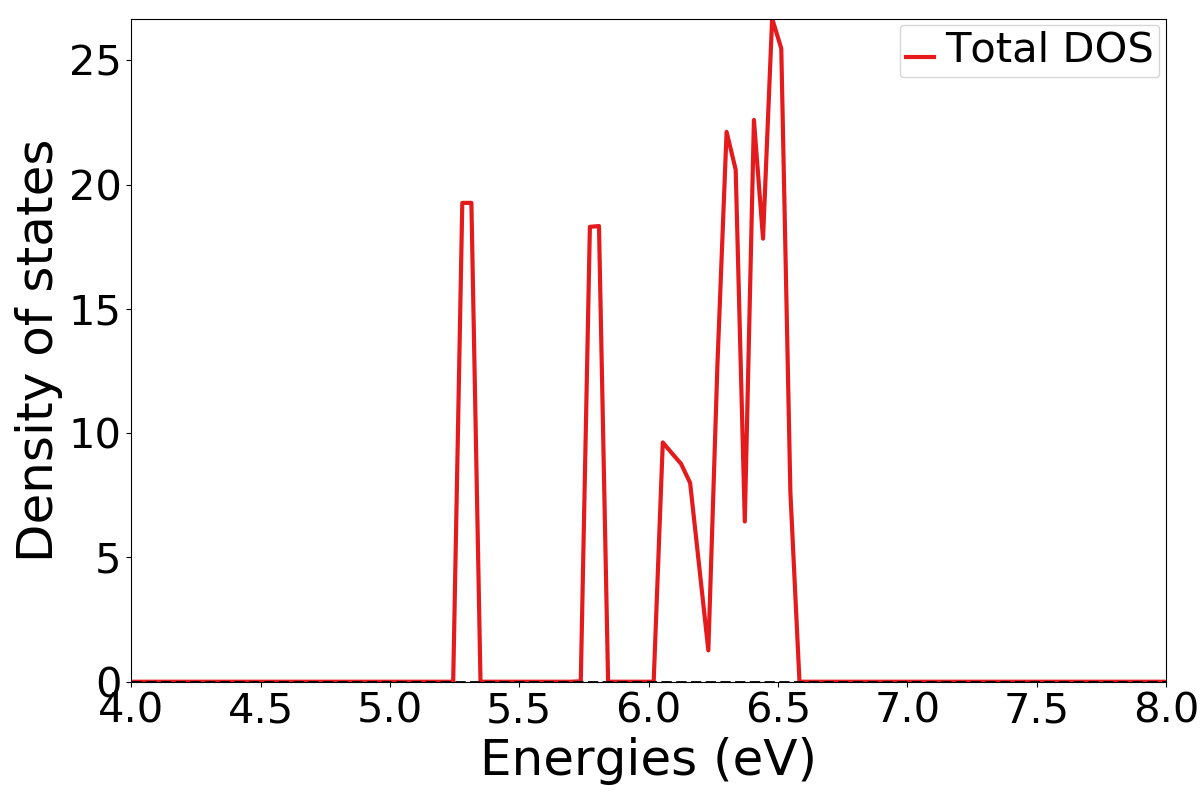
\includegraphics[width = 11cm]{../fig/DOS_k4_TDOS_2.png}
      \caption{. }
      \label{fig:DOS_k4_TDOS_2}
  \end{figure}

  \begin{figure}[H]
      \centering
      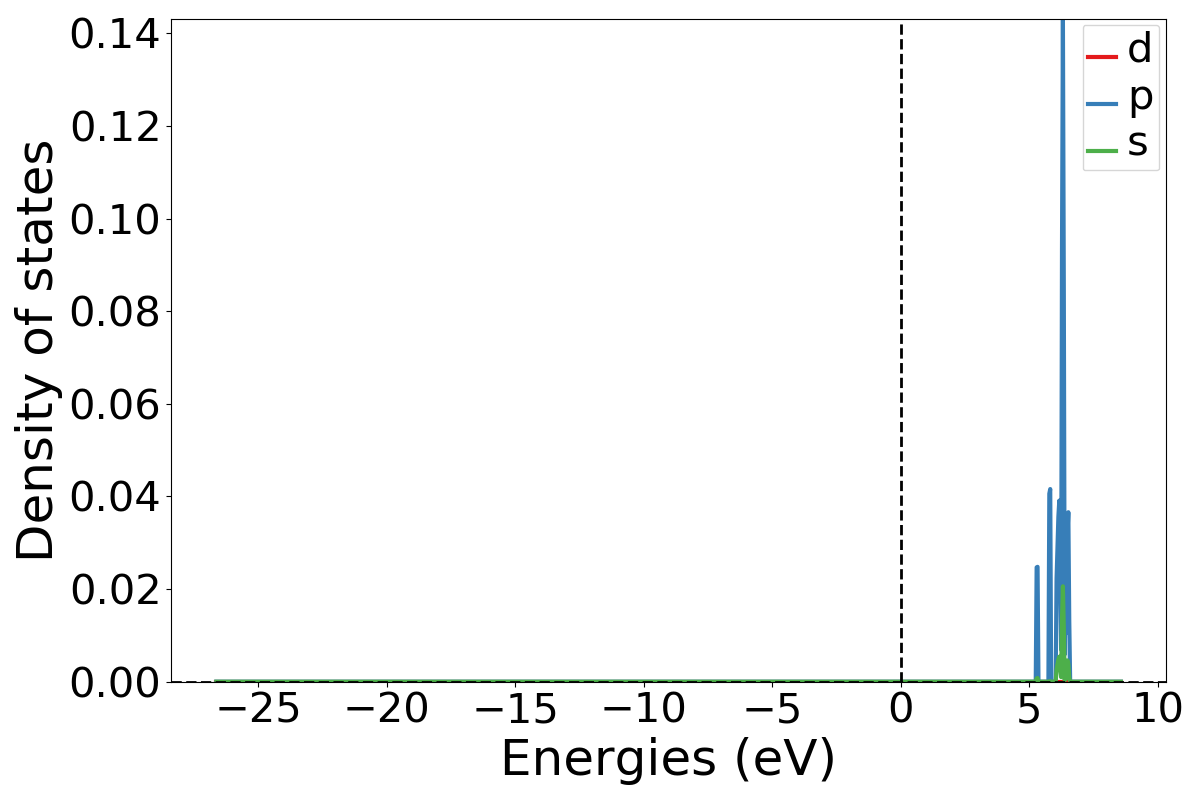
\includegraphics[width = 11cm]{../fig/DOS_k4_LDOS25_1.png}
      \caption{.}
      \label{fig:DOS_k4_LDOS25_1}
  \end{figure}

  \begin{figure}[H]
      \centering
      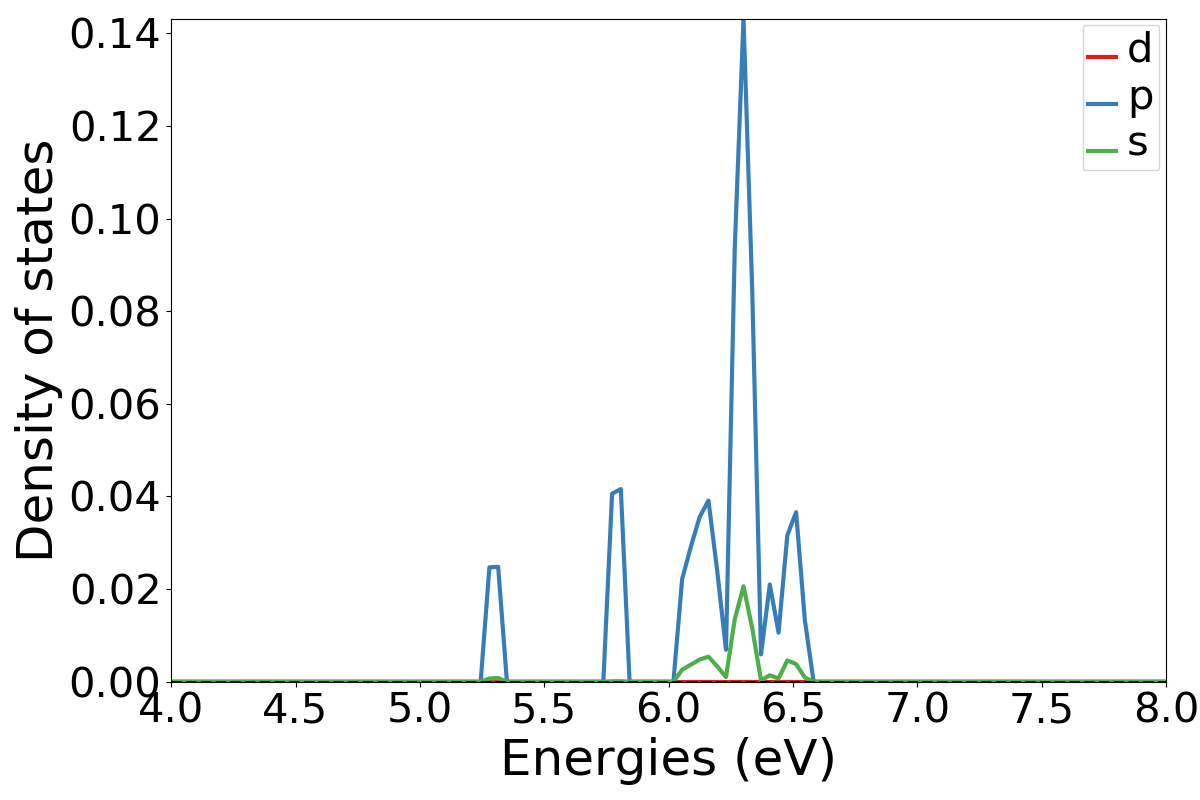
\includegraphics[width = 11cm]{../fig/DOS_k4_LDOS25_2.png}
      \caption{. }
      \label{fig:DOS_k4_LDOS25_2}
  \end{figure}

  \begin{figure}[H]
      \centering
      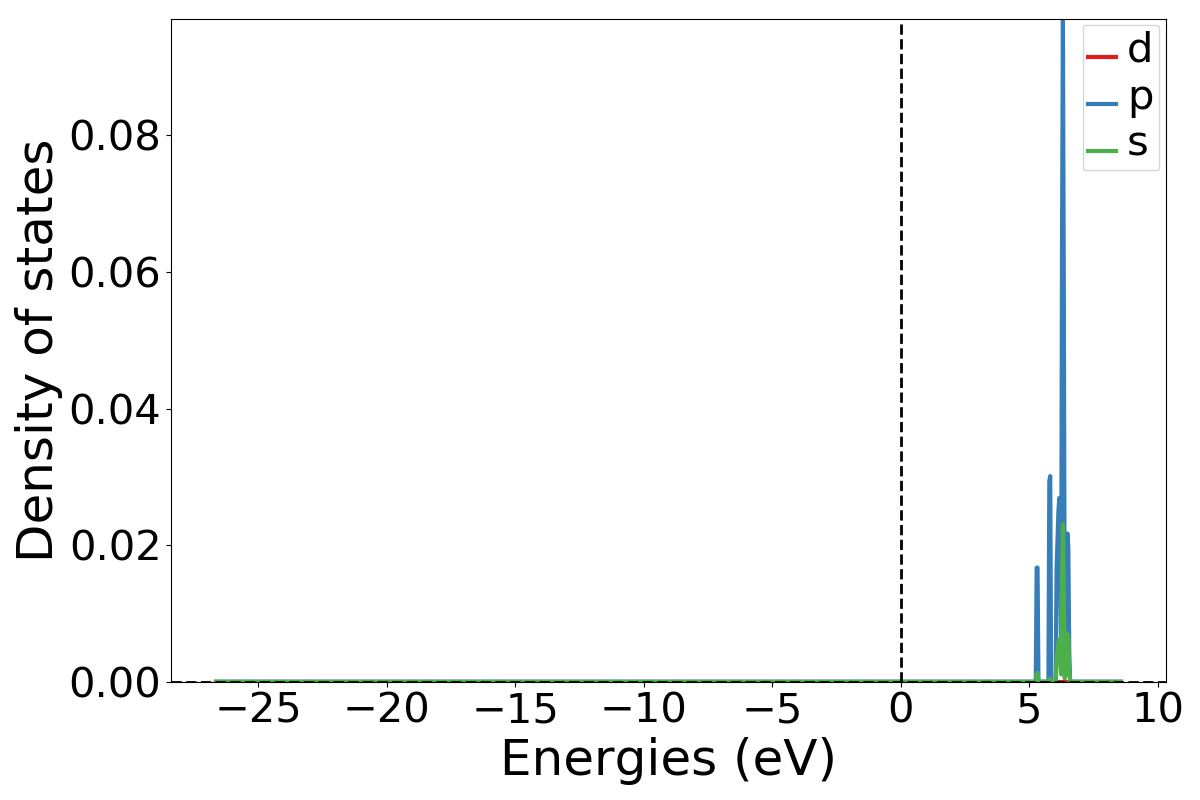
\includegraphics[width = 11cm]{../fig/DOS_k4_LDOS26_1.png}
      \caption{. }
      \label{fig:DOS_k4_LDOS26_1}
  \end{figure}

  \begin{figure}[H]
      \centering
      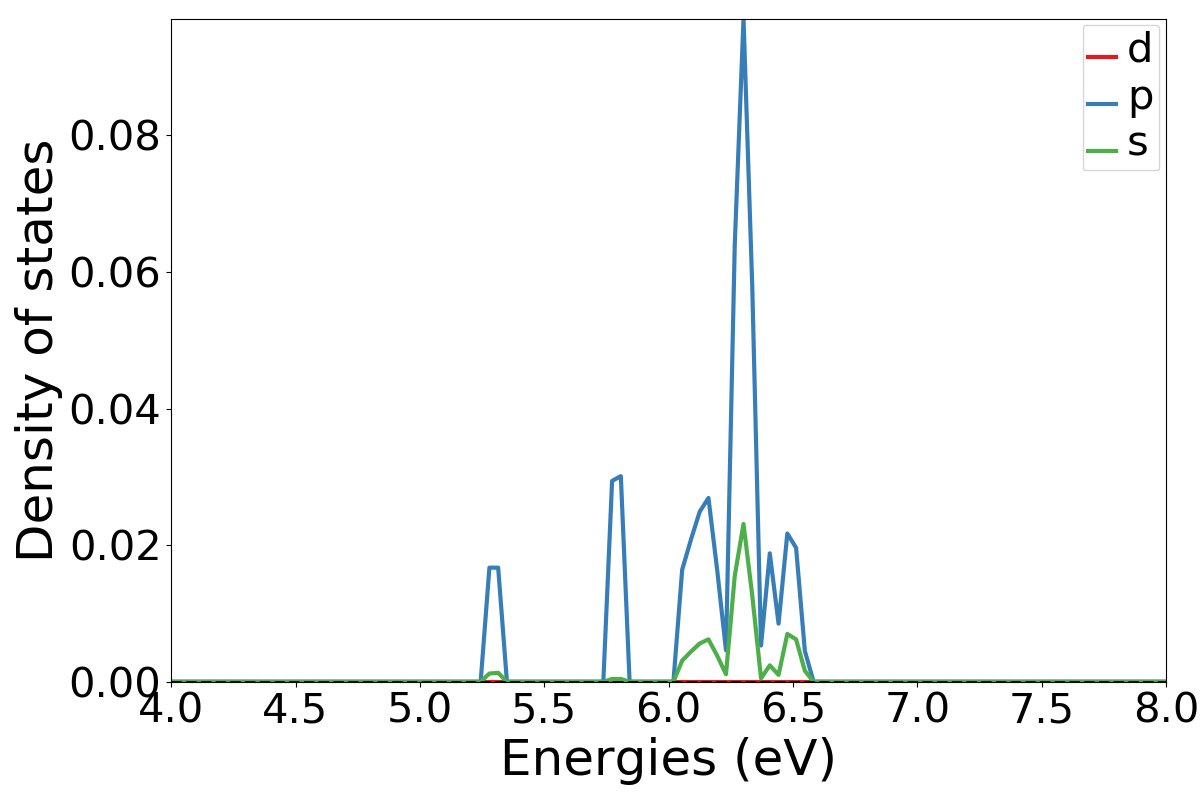
\includegraphics[width = 11cm]{../fig/DOS_k4_LDOS26_2.png}
      \caption{. }
      \label{fig:DOS_k4_LDOS26_2}
  \end{figure}

\vspace{1cm}

\section{Y-bilder}

  \begin{figure}[H]
      \centering
      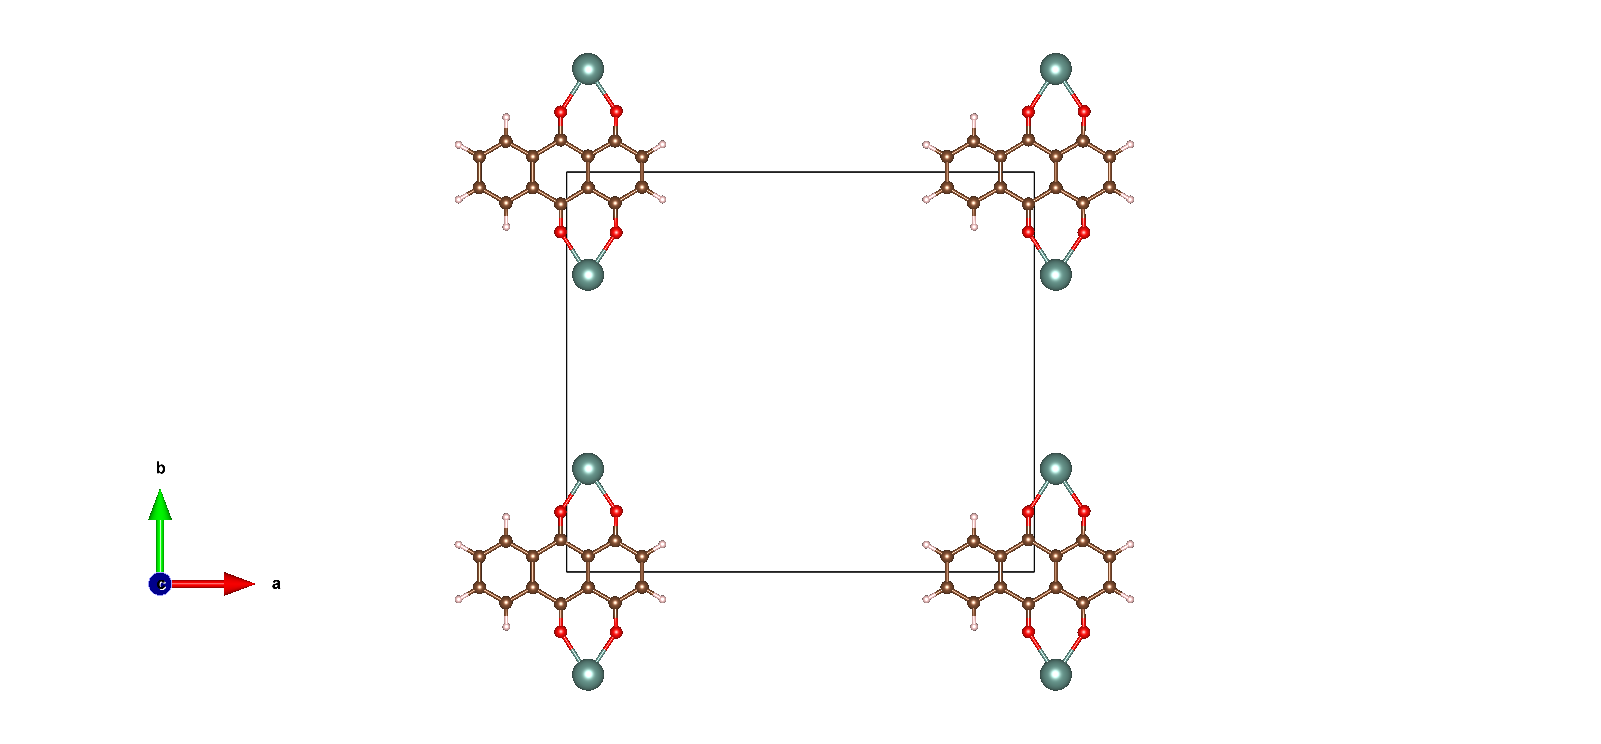
\includegraphics[width = 11cm]{../fig/Y_staticbefore_CONTCAR.png}
      \caption{. }
      \label{fig:Y_staticbefore_CONTCAR}
  \end{figure}

  \begin{figure}[H]
      \centering
      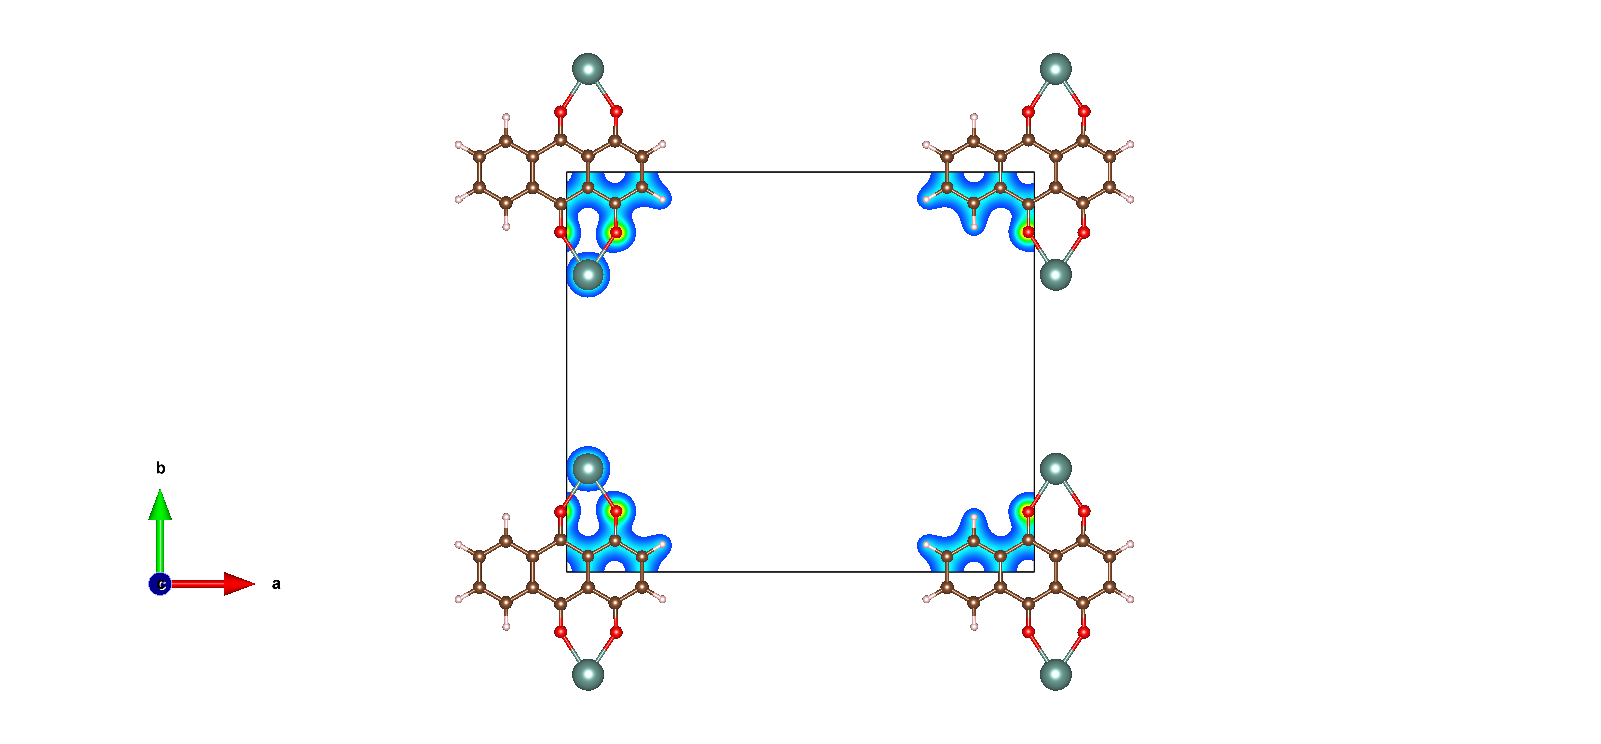
\includegraphics[width = 11cm]{../fig/Y_staticbefore_CHGCAR.png}
      \caption{. }
      \label{fig:Y_staticbefore_CHGCAR}
  \end{figure}

  \begin{figure}[H]
      \centering
      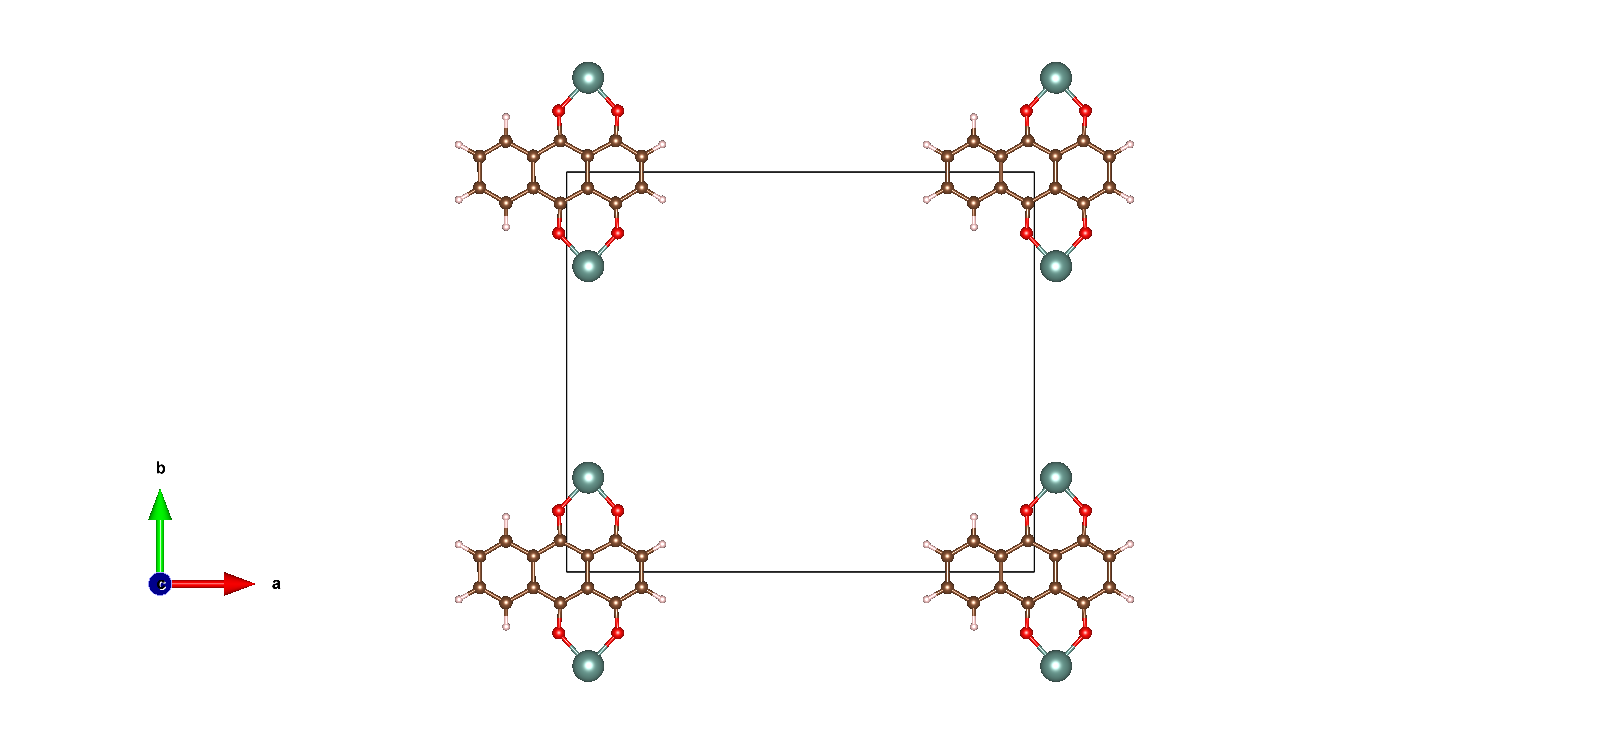
\includegraphics[width = 11cm]{../fig/Y_relax_CONTCAR.png}
      \caption{. }
      \label{fig:Y_relax_CONTCAR}
  \end{figure}

  \begin{figure}[H]
      \centering
      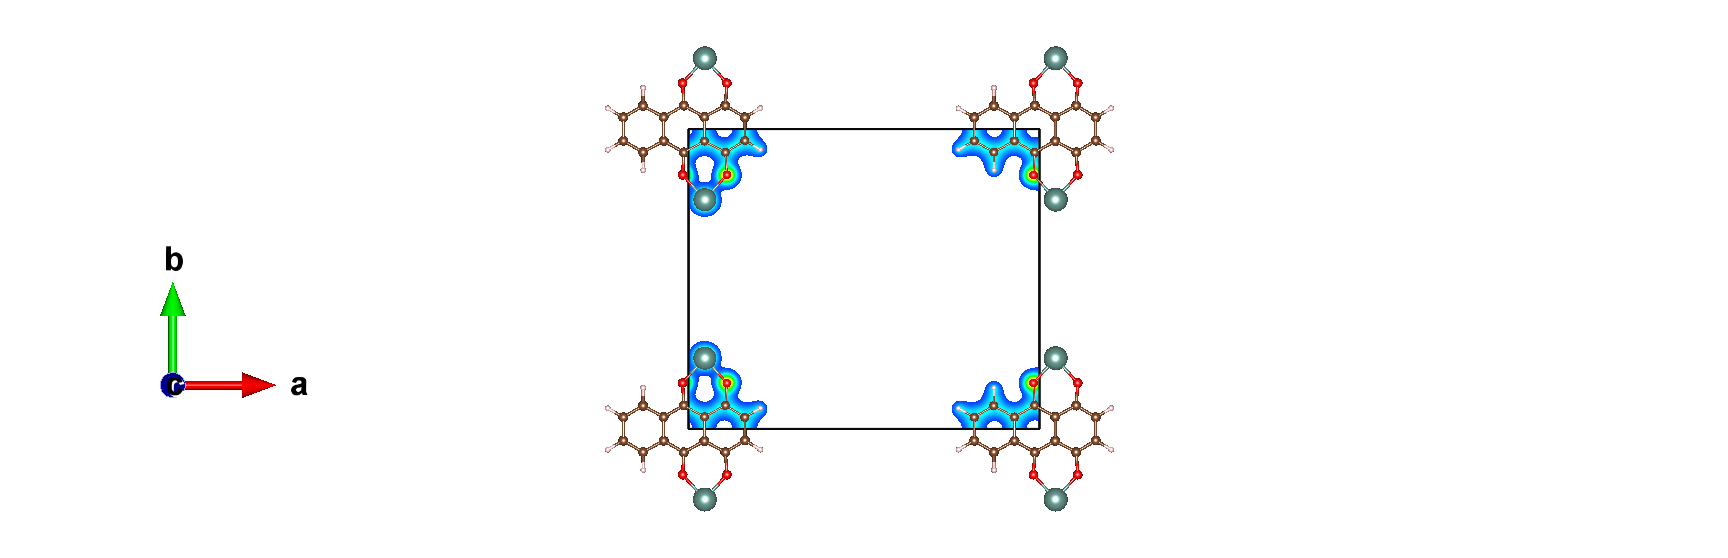
\includegraphics[width = 11cm]{../fig/Y_relax_CHGCAR.png}
      \caption{. }
      \label{fig:Y_relax_CHGCAR}
  \end{figure}

  \iffalse
  \begin{figure}[H]
      \centering
      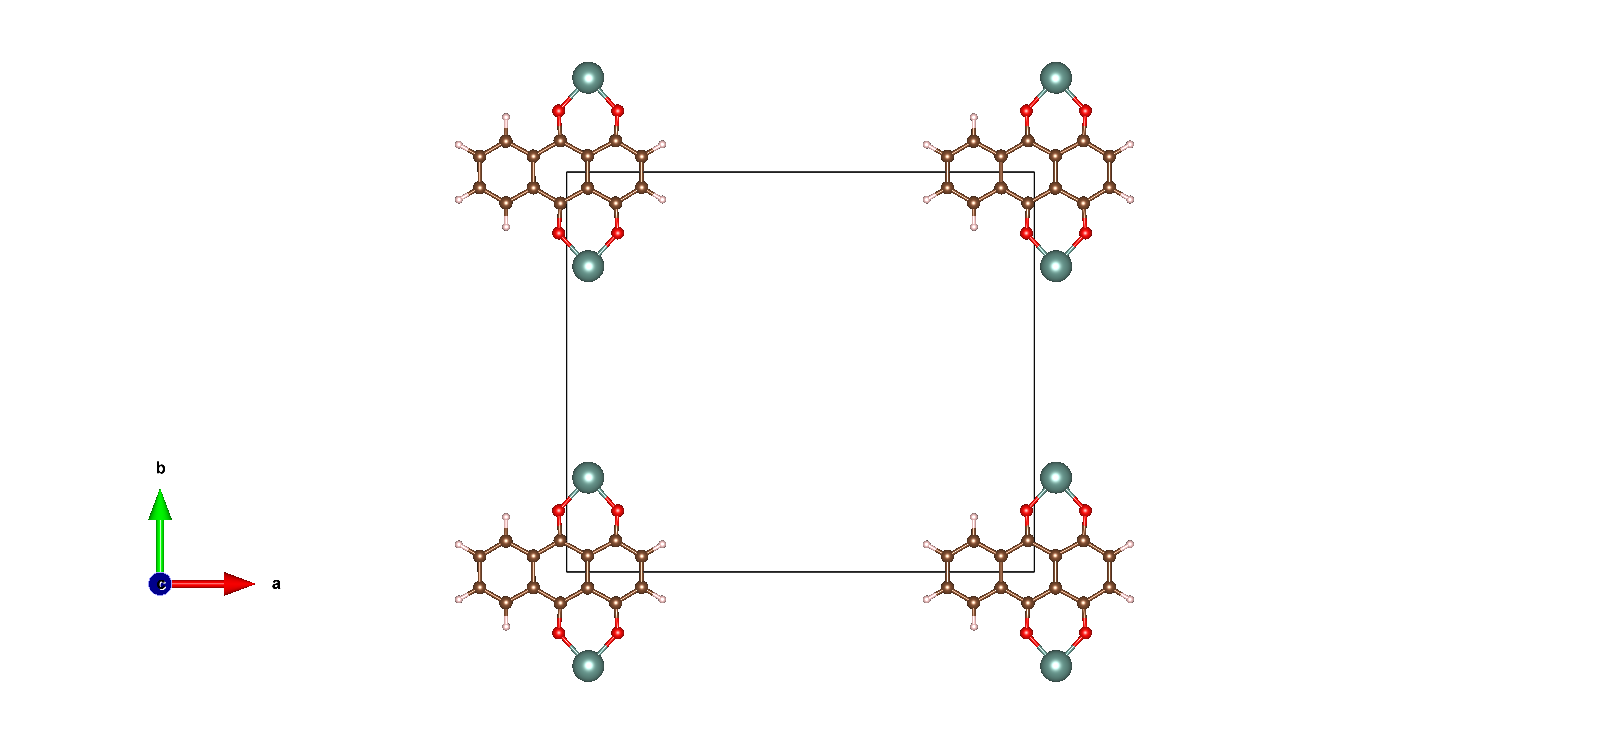
\includegraphics[width = 11cm]{../fig/Y_staticafter_CONTCAR.png}
      \caption{. }
      \label{fig:Y_staticafter_CONTCAR}
  \end{figure}

  \begin{figure}[H]
      \centering
      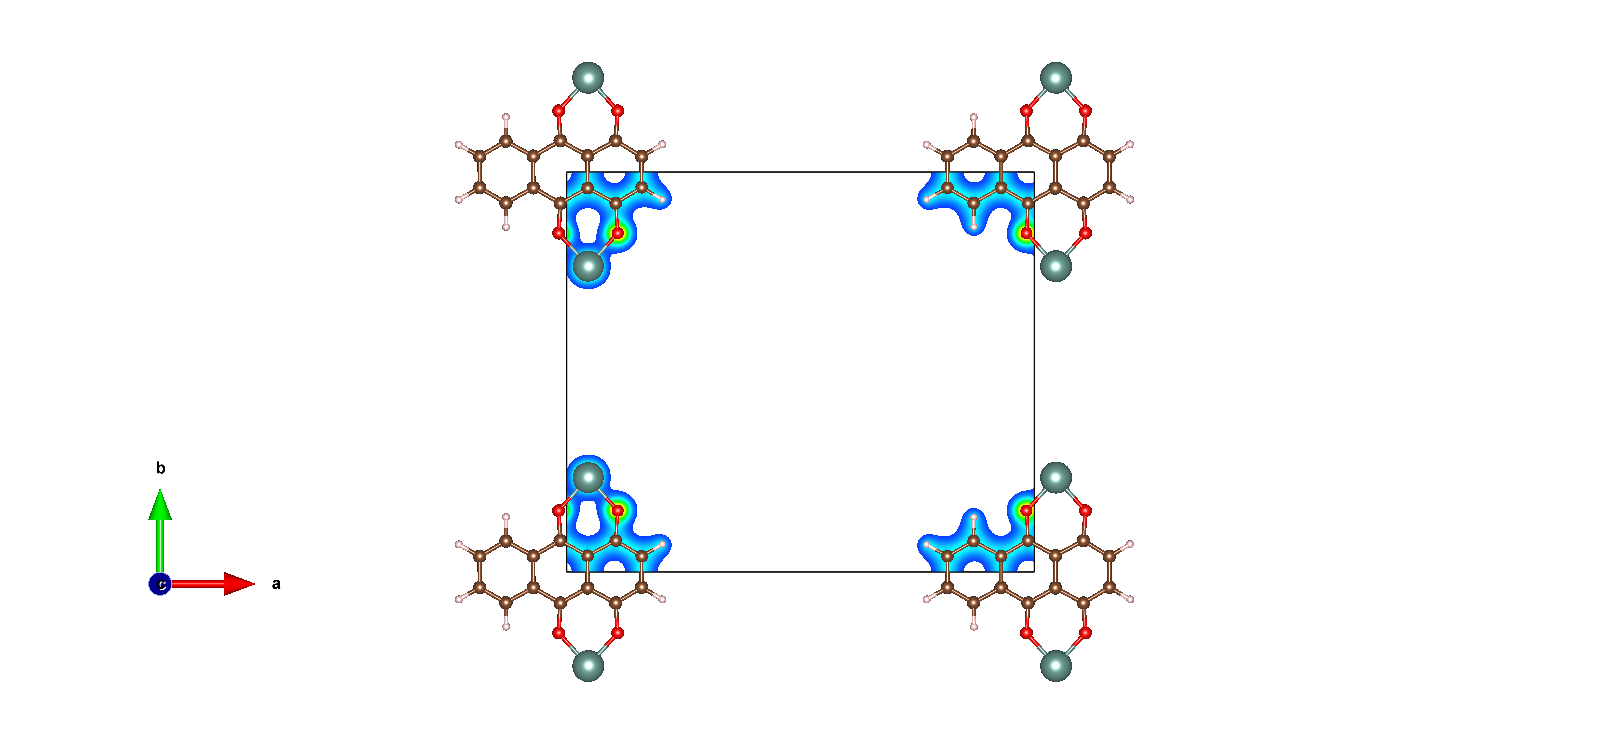
\includegraphics[width = 11cm]{../fig/Y_staticafter_CHGCAR.png}
      \caption{. }
      \label{fig:Y_staticafter_CHGCAR}
  \end{figure}
  \fi

  \begin{figure}[H]
      \centering
      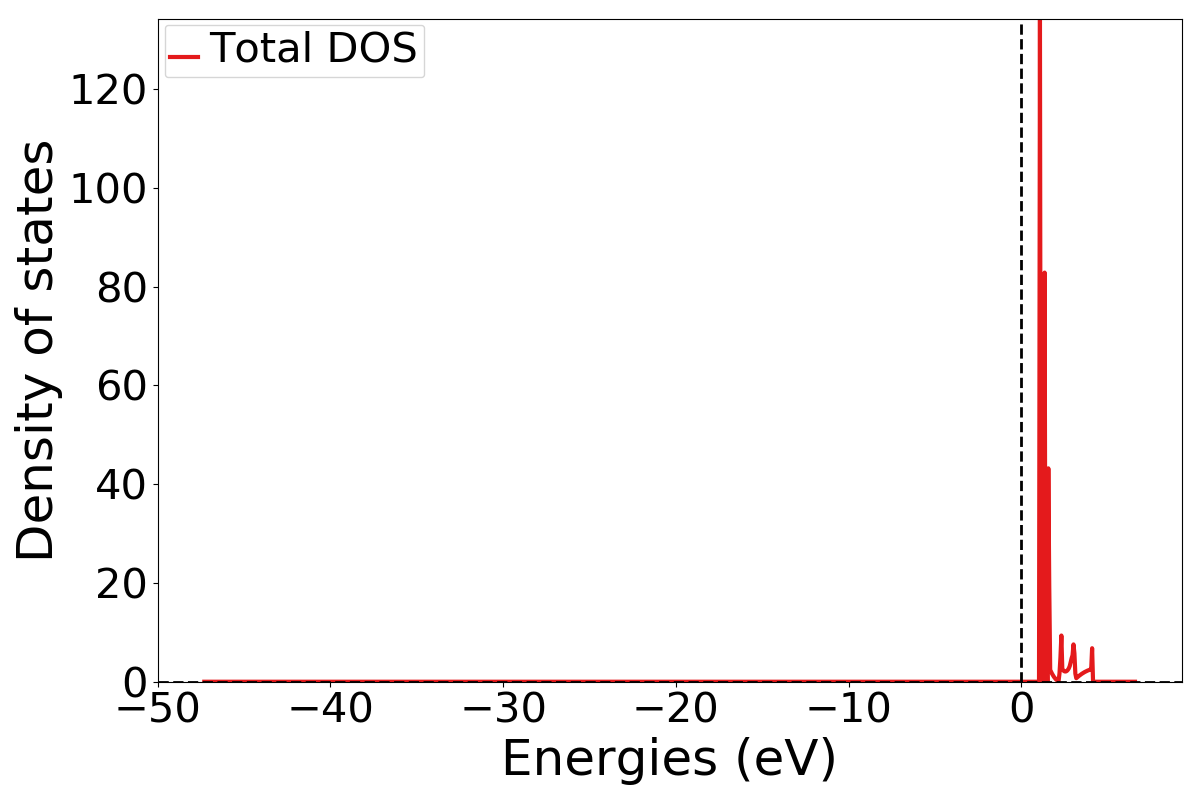
\includegraphics[width = 11cm]{../fig/Y_k4_TDOS_1.png}
      \caption{. }
      \label{fig:Y_k4_TDOS_1.png}
  \end{figure}

  \begin{figure}[H]
      \centering
      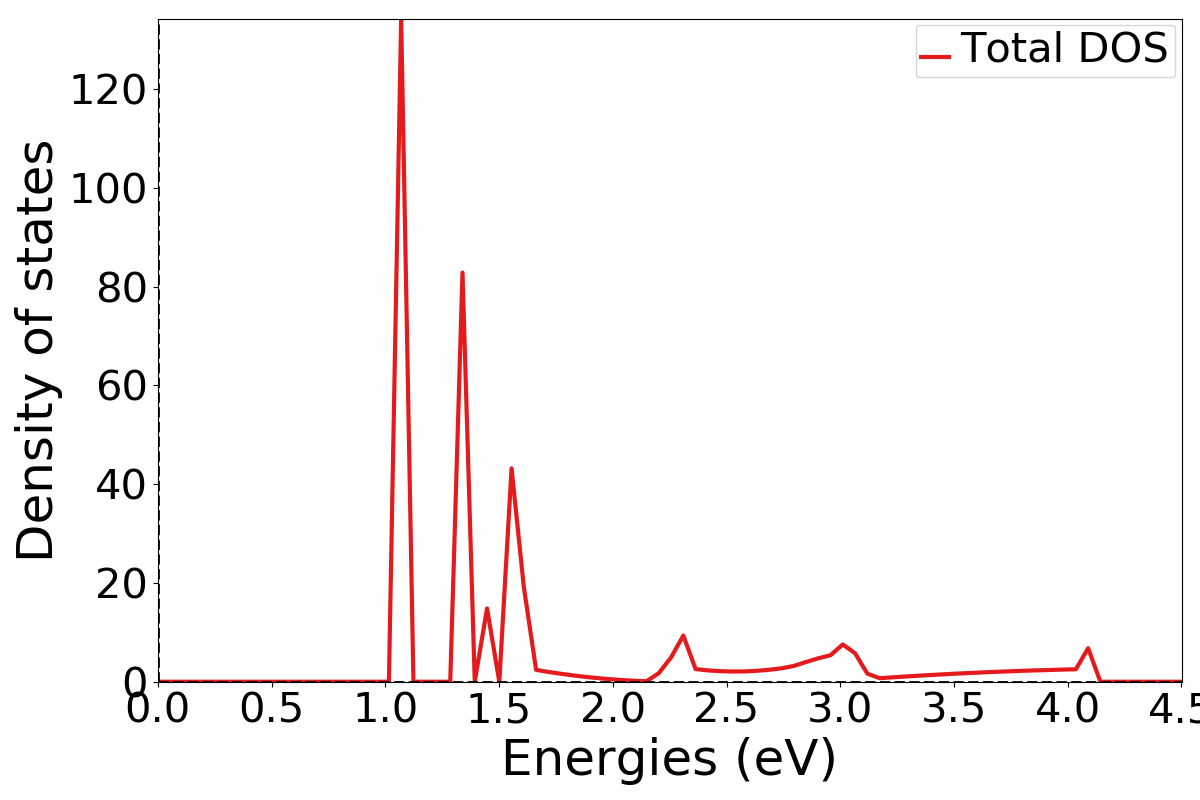
\includegraphics[width = 11cm]{../fig/Y_k4_TDOS_2.png}
      \caption{. }
      \label{fig:Y_k4_TDOS_2.png}
  \end{figure}

  \begin{figure}[H]
      \centering
      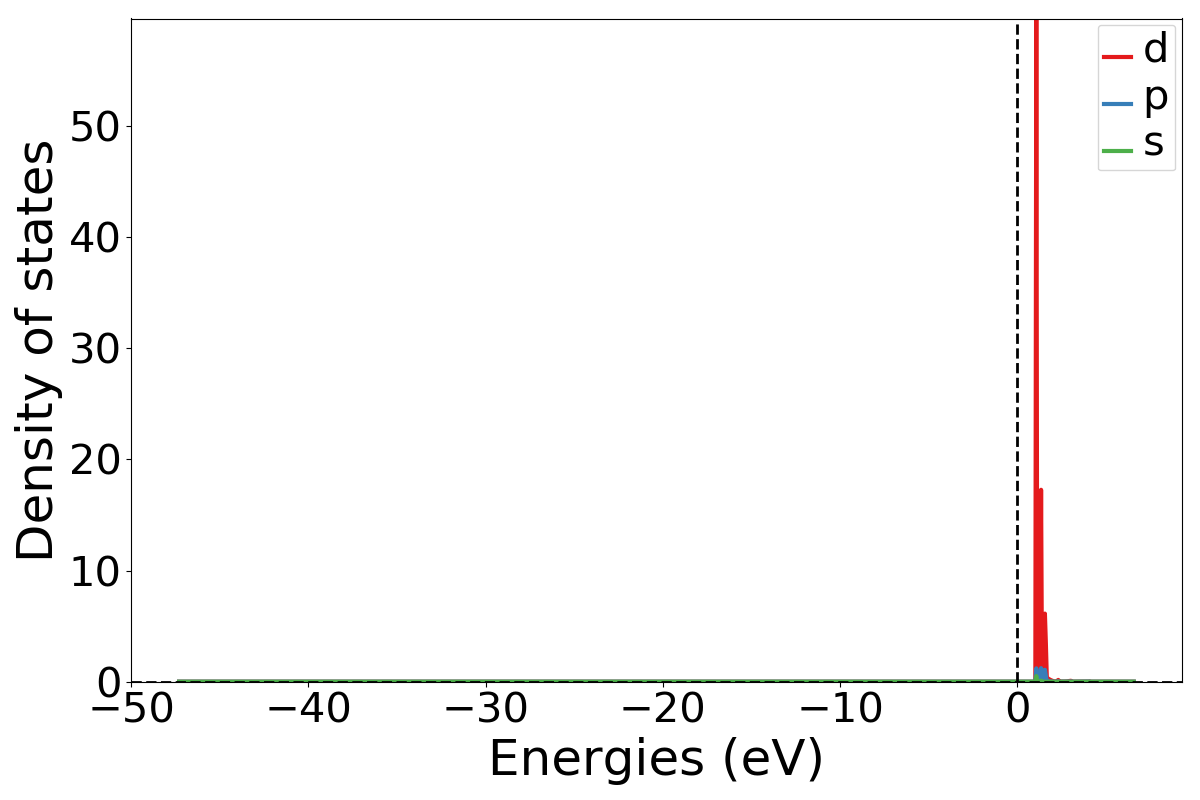
\includegraphics[width = 11cm]{../fig/Y_k4_LDOS25_1.png}
      \caption{. }
      \label{fig:Y_k4_LDOS25_1.png}
  \end{figure}

  \begin{figure}[H]
      \centering
      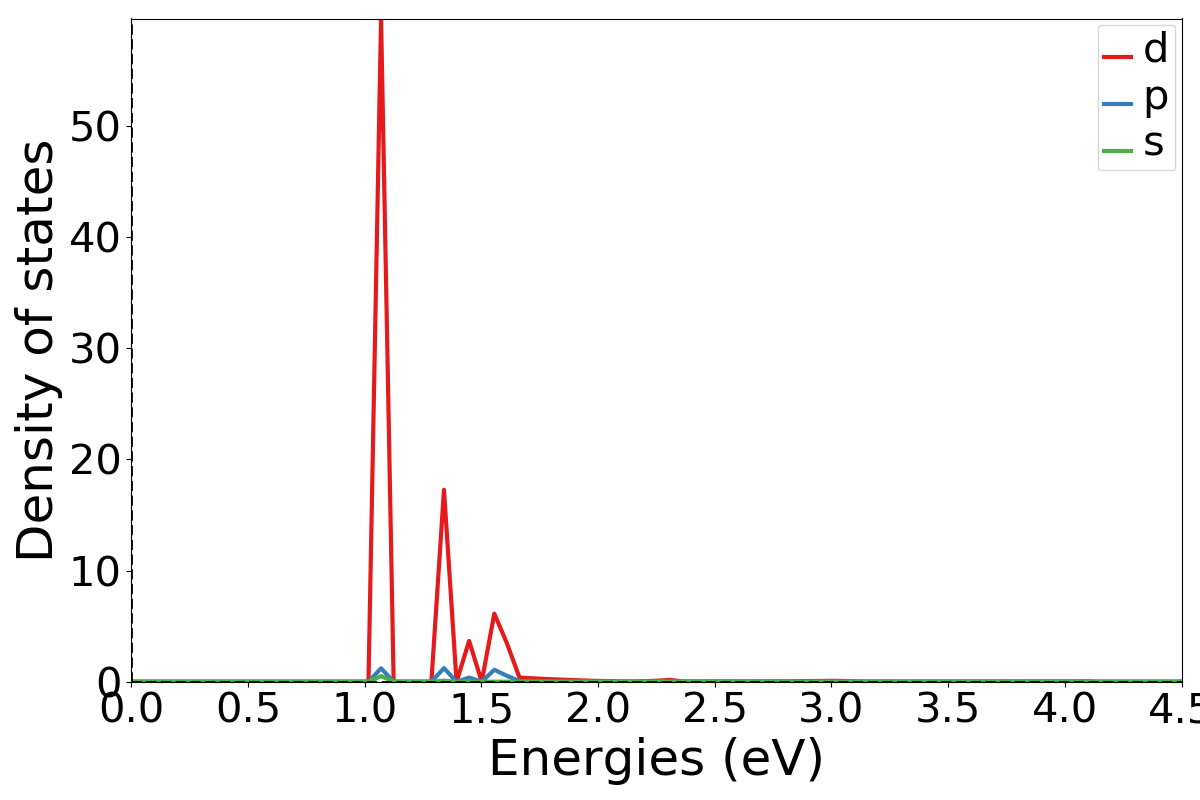
\includegraphics[width = 11cm]{../fig/Y_k4_LDOS25_2.png}
      \caption{. }
      \label{fig:Y_k4_LDOS25_2.png}
  \end{figure}

  \begin{figure}[H]
      \centering
      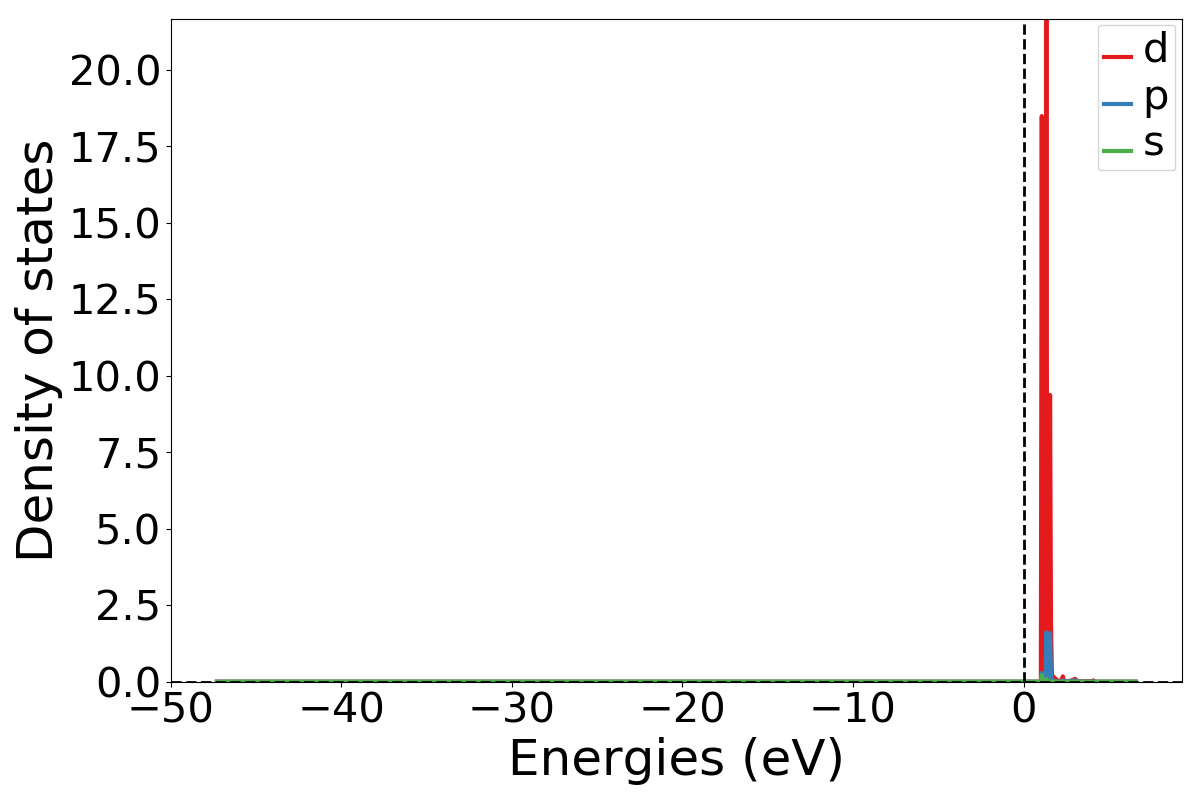
\includegraphics[width = 11cm]{../fig/Y_k4_LDOS26_1.png}
      \caption{. }
      \label{fig:Y_k4_LDOS26_1.png}
  \end{figure}

  \begin{figure}[H]
      \centering
      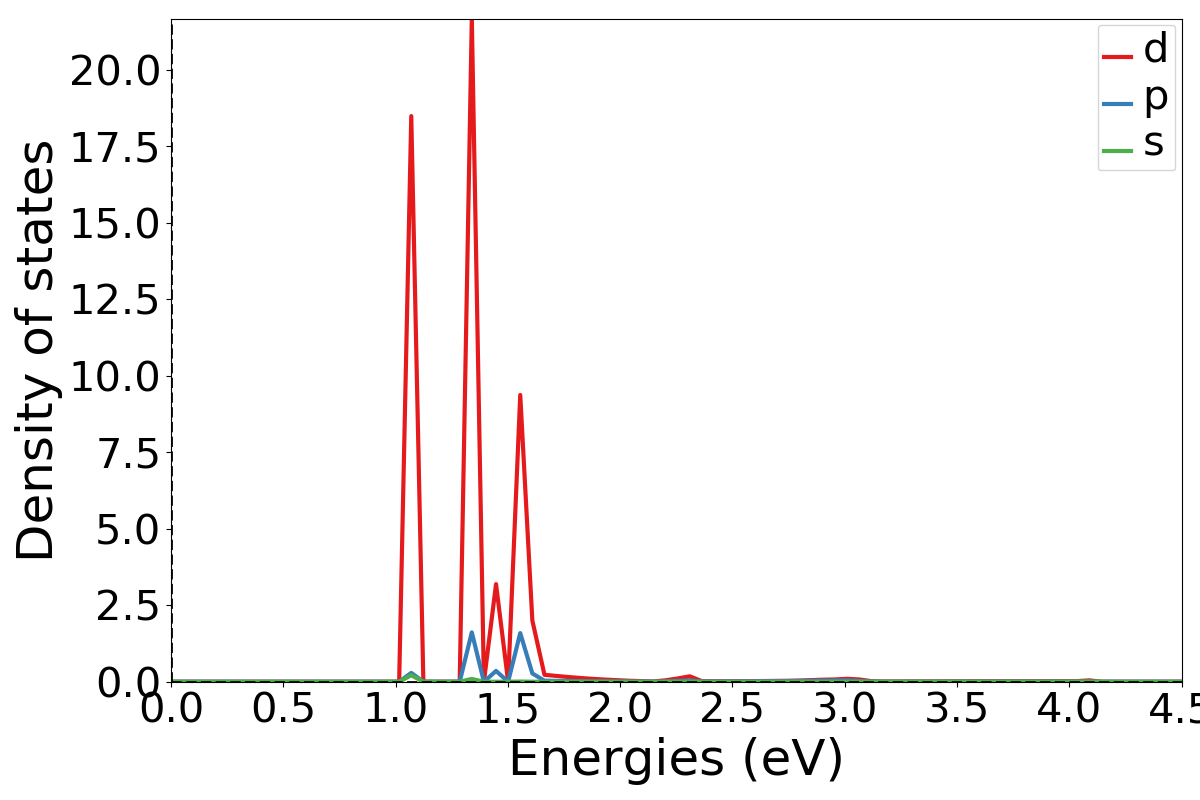
\includegraphics[width = 11cm]{../fig/Y_k4_LDOS26_2.png}
      \caption{. }
      \label{fig:Y_k4_LDOS26_2.png}
  \end{figure}

\vspace{1cm}

\section{Yb-bilder}

  \begin{figure}[H]
      \centering
      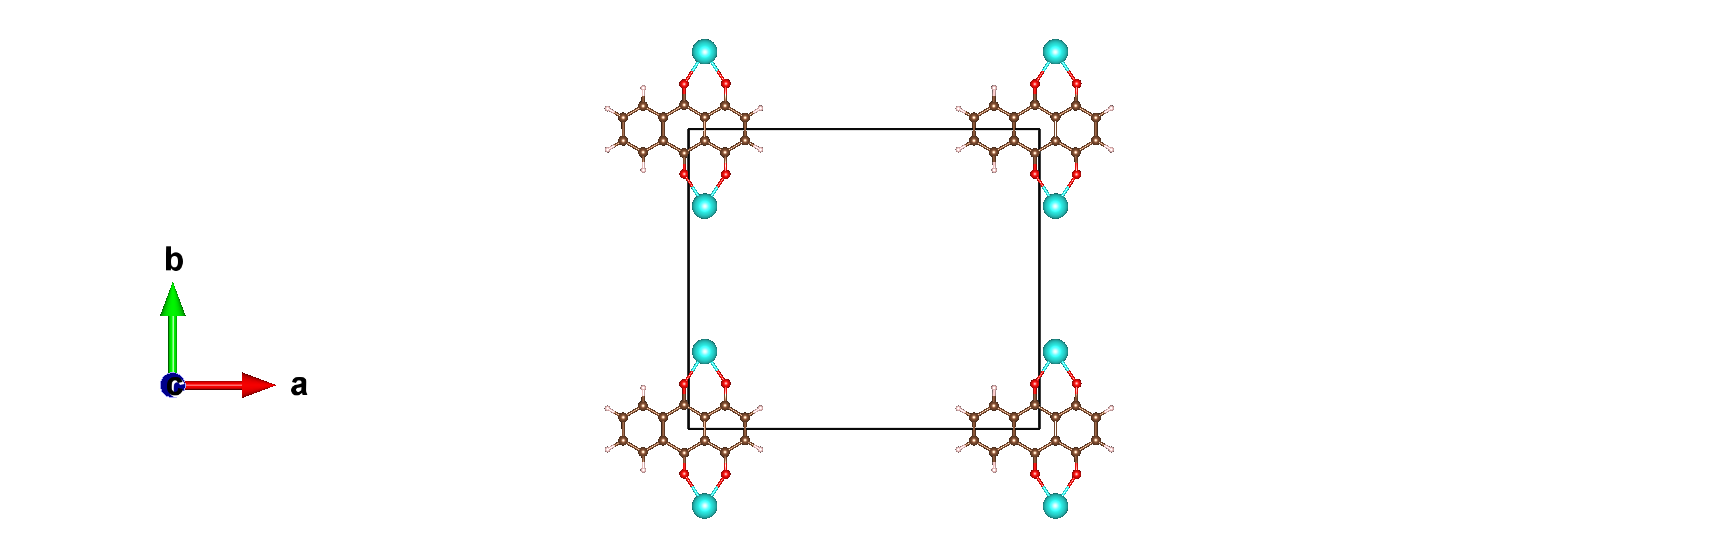
\includegraphics[width = 11cm]{../fig/Yb_staticbefore_CONTCAR.png}
      \caption{. }
      \label{fig:Yb_staticbefore_CONTCAR}
  \end{figure}

  \begin{figure}[H]
      \centering
      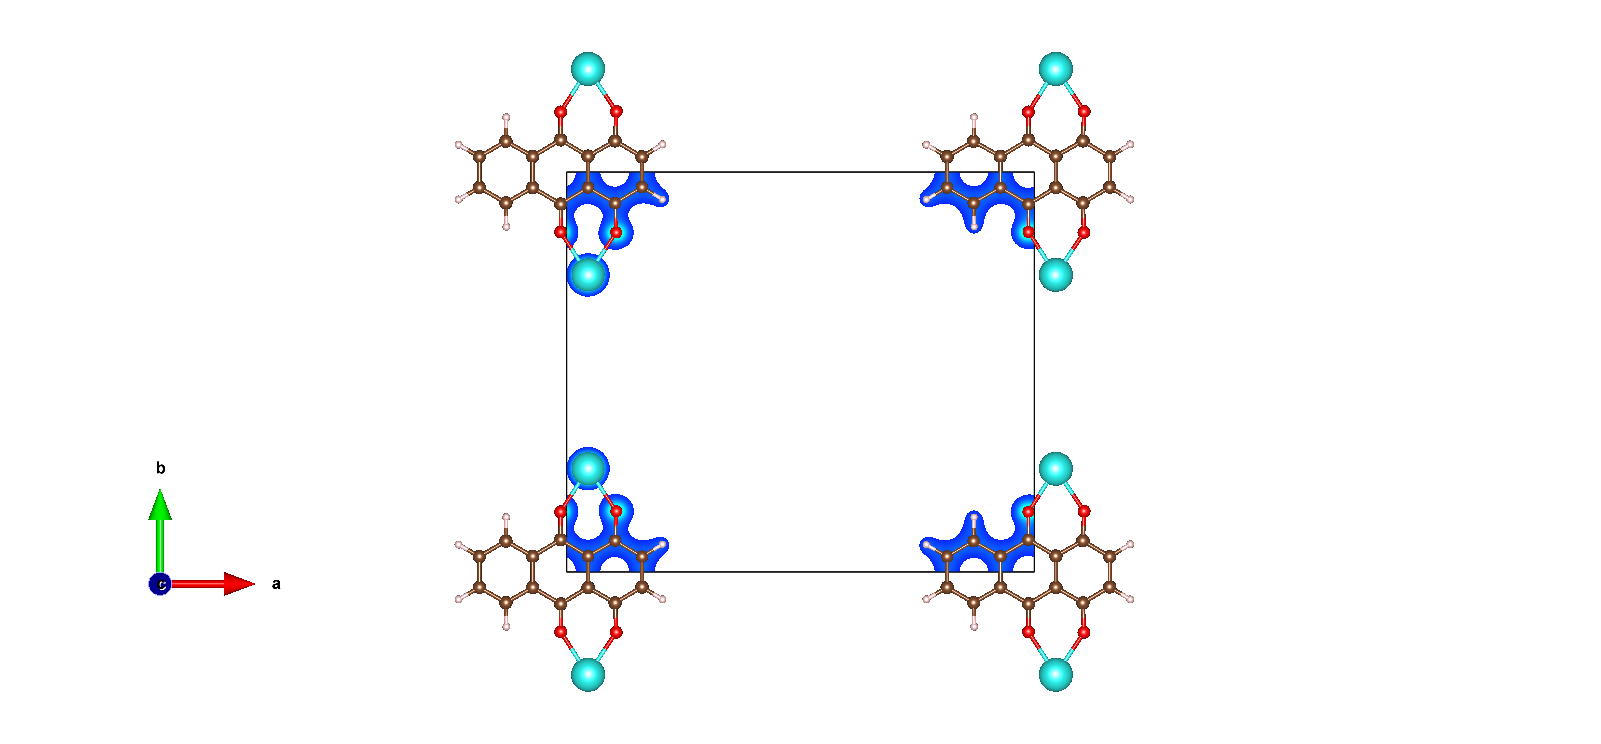
\includegraphics[width = 11cm]{../fig/Yb_staticbefore_CHGCAR.png}
      \caption{. }
      \label{fig:Yb_staticbefore_CHGCAR}
  \end{figure}

  \begin{figure}[H]
      \centering
      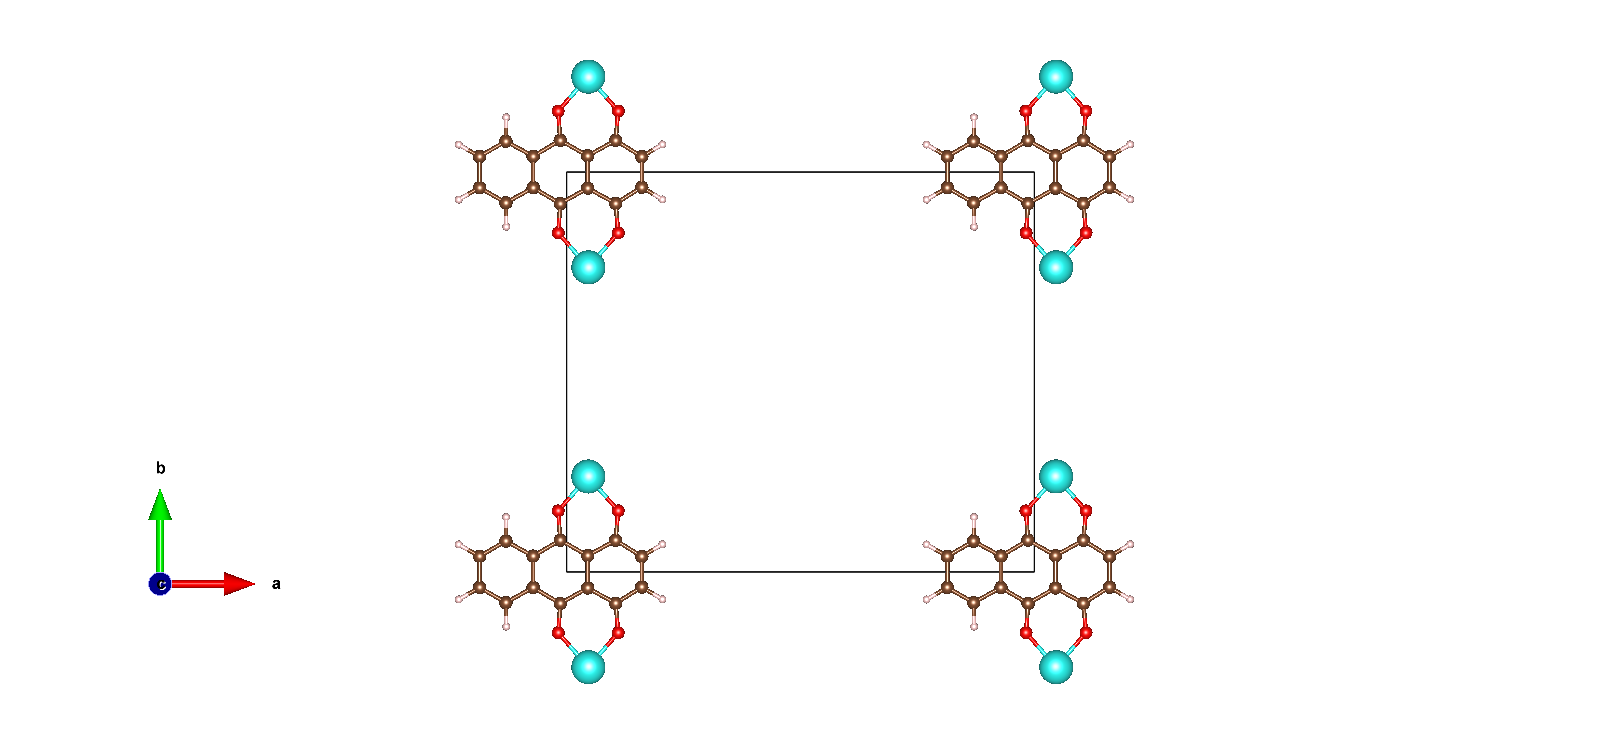
\includegraphics[width = 11cm]{../fig/Yb_relax_CONTCAR.png}
      \caption{. }
      \label{fig:Yb_relax_CONTCAR}
  \end{figure}

  \begin{figure}[H]
      \centering
      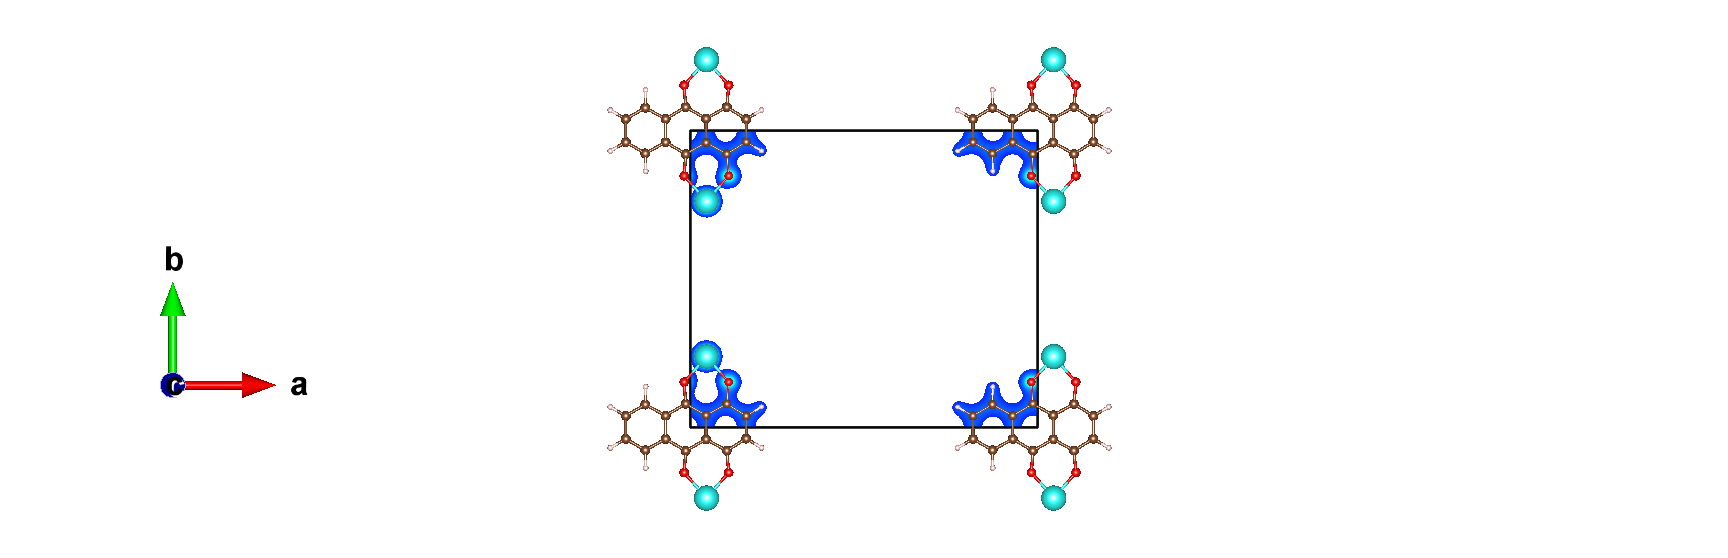
\includegraphics[width = 11cm]{../fig/Yb_relax_CHGCAR.png}
      \caption{. }
      \label{fig:Yb_relax_CHGCAR}
  \end{figure}

  \iffalse
  \begin{figure}[H]
      \centering
      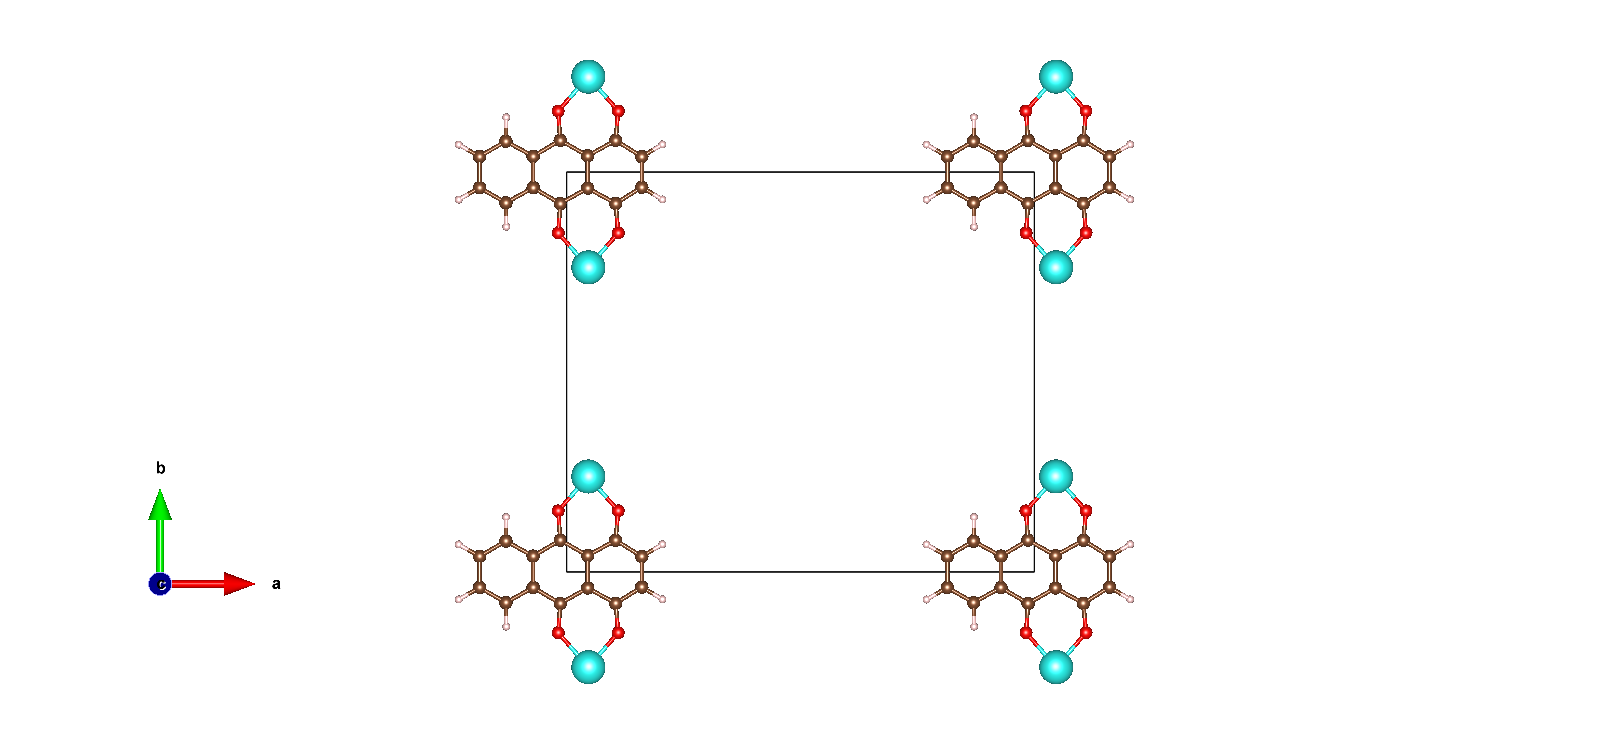
\includegraphics[width = 11cm]{../fig/Yb_staticafter_CONTCAR.png}
      \caption{. }
      \label{fig:Yb_staticafter_CONTCAR}
  \end{figure}

  \begin{figure}[H]
      \centering
      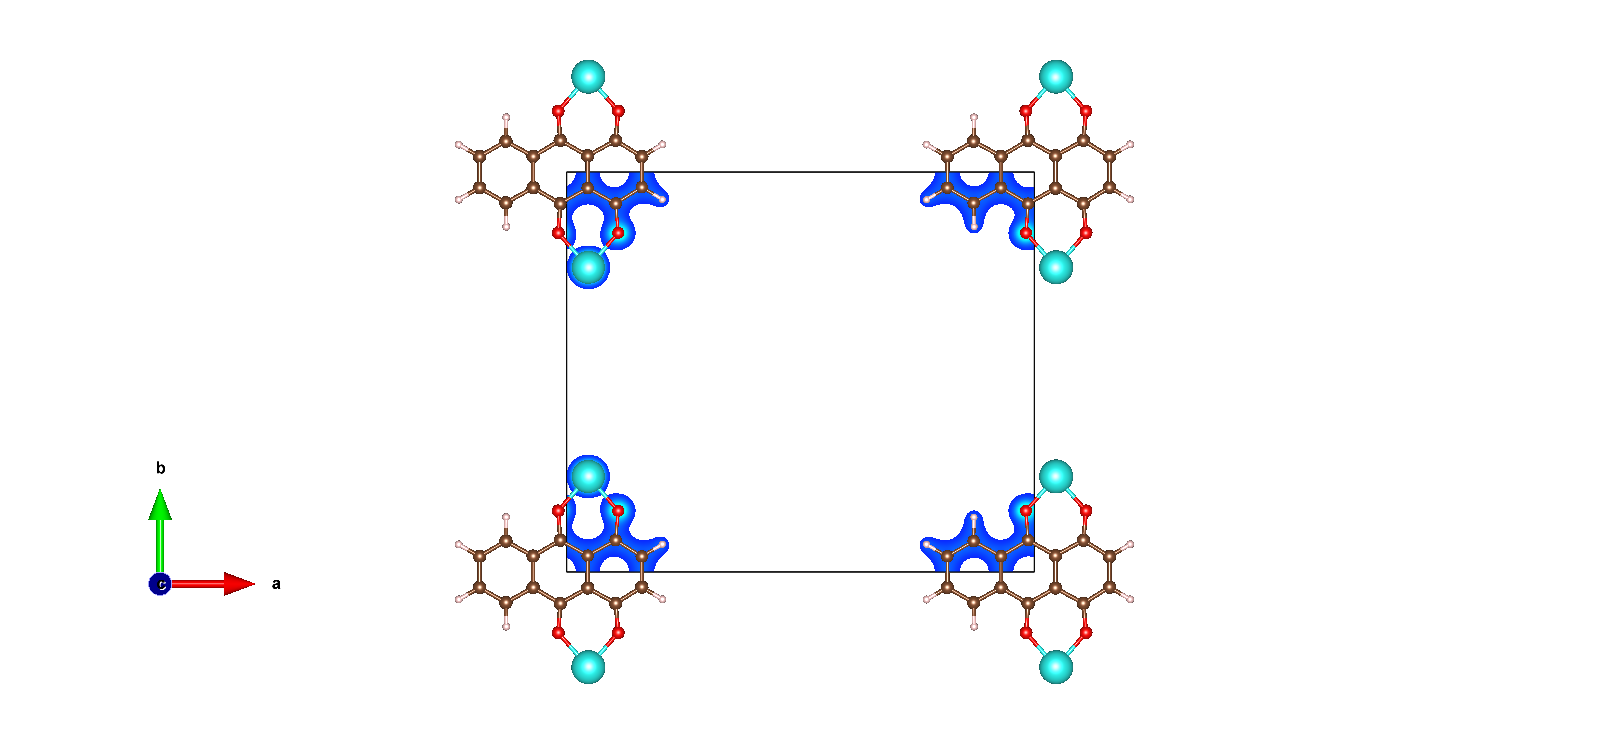
\includegraphics[width = 11cm]{../fig/Yb_staticafter_CHGCAR.png}
      \caption{. }
      \label{fig:Yb_staticafter_CHGCAR}
  \end{figure}
  \fi

  \begin{figure}[H]
      \centering
      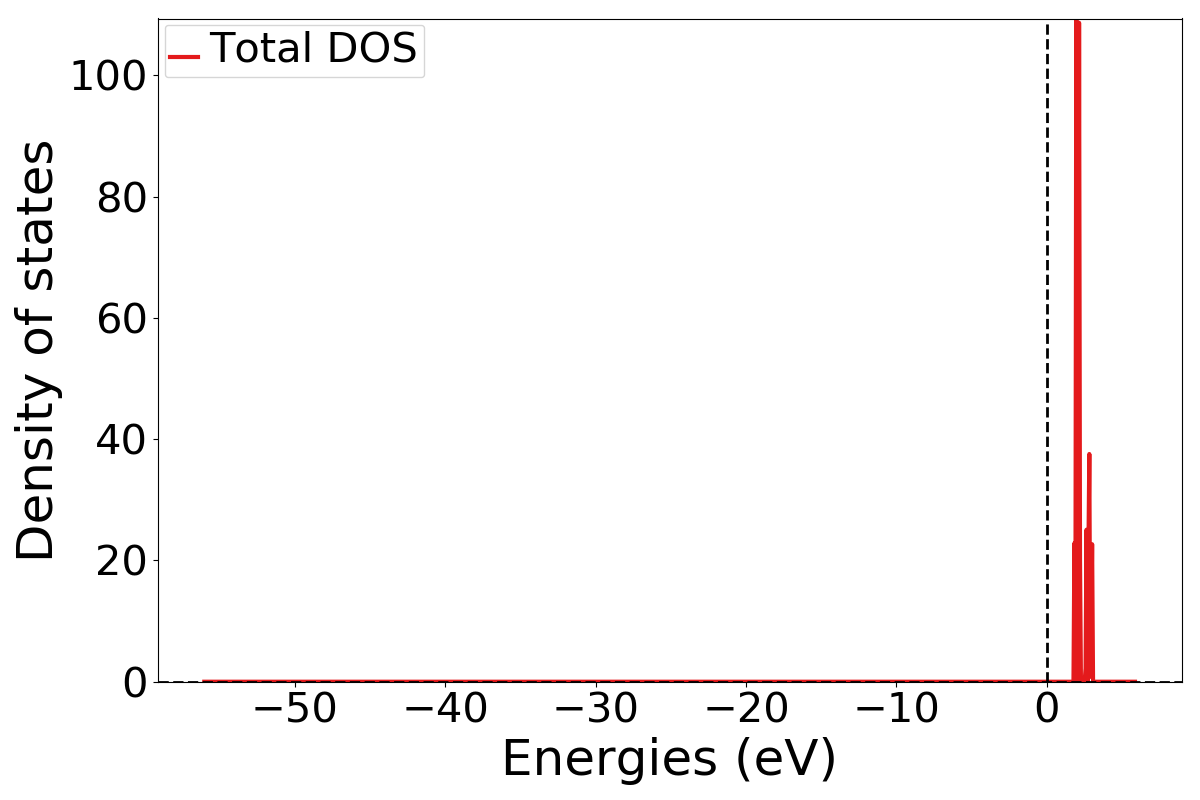
\includegraphics[width = 11cm]{../fig/Yb_k4_TDOS_1.png}
      \caption{. }
      \label{fig:Yb_k4_TDOS_1.png}
  \end{figure}

  \begin{figure}[H]
      \centering
      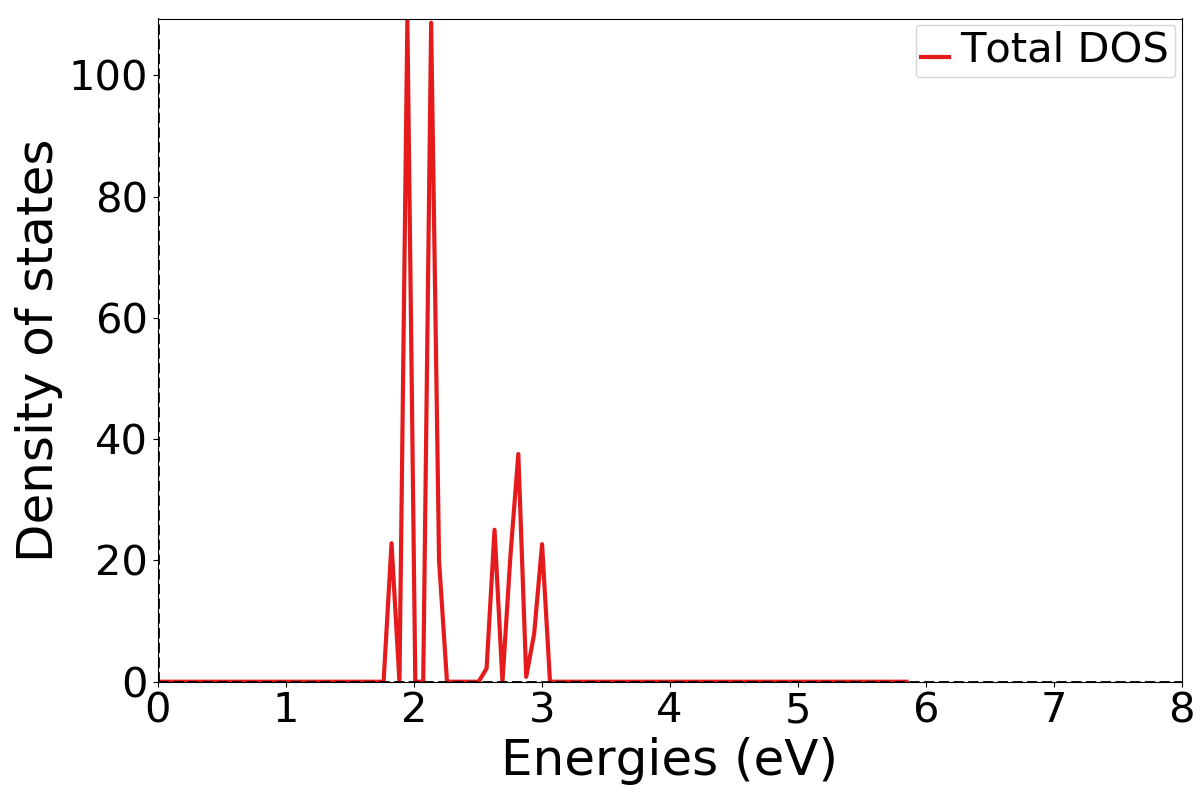
\includegraphics[width = 11cm]{../fig/Yb_k4_TDOS_2.png}
      \caption{. }
      \label{fig:Yb_k4_TDOS_2.png}
  \end{figure}

  \begin{figure}[H]
      \centering
      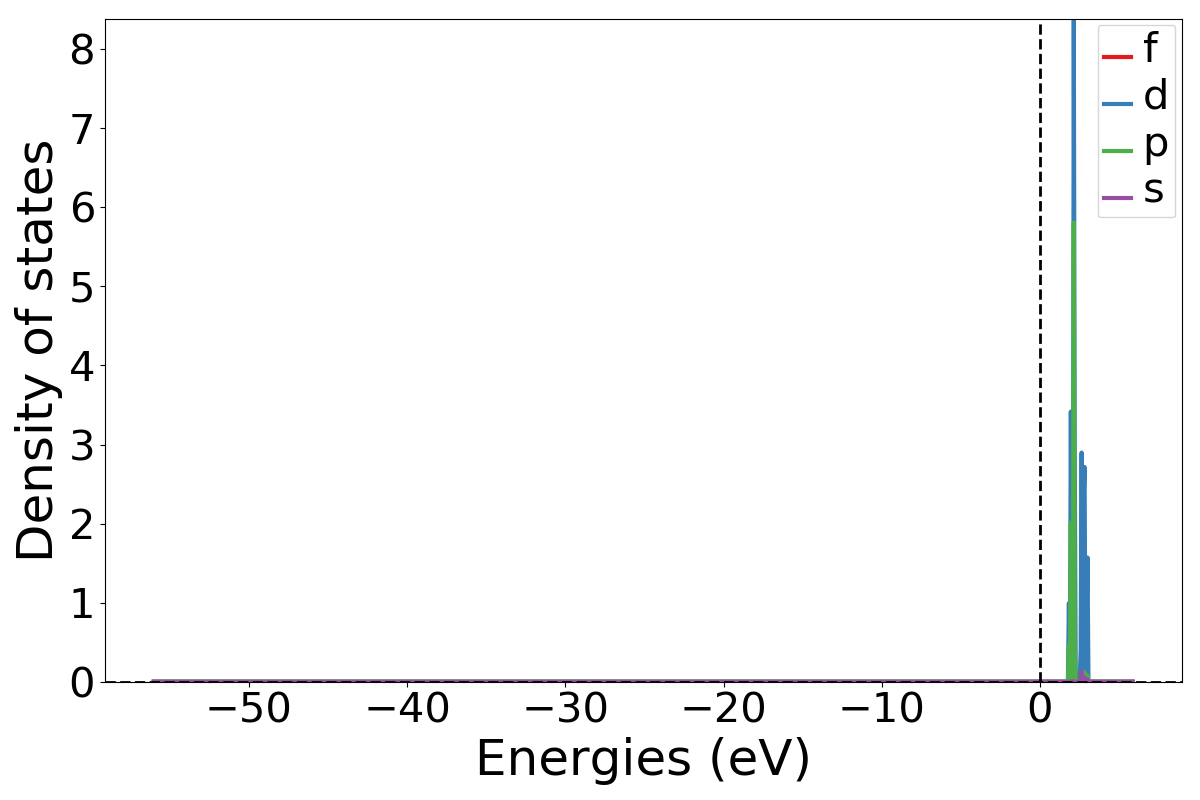
\includegraphics[width = 11cm]{../fig/Yb_k4_LDOS25_1.png}
      \caption{. }
      \label{fig:Yb_k4_LDOS25_1.png}
  \end{figure}

  \begin{figure}[H]
      \centering
      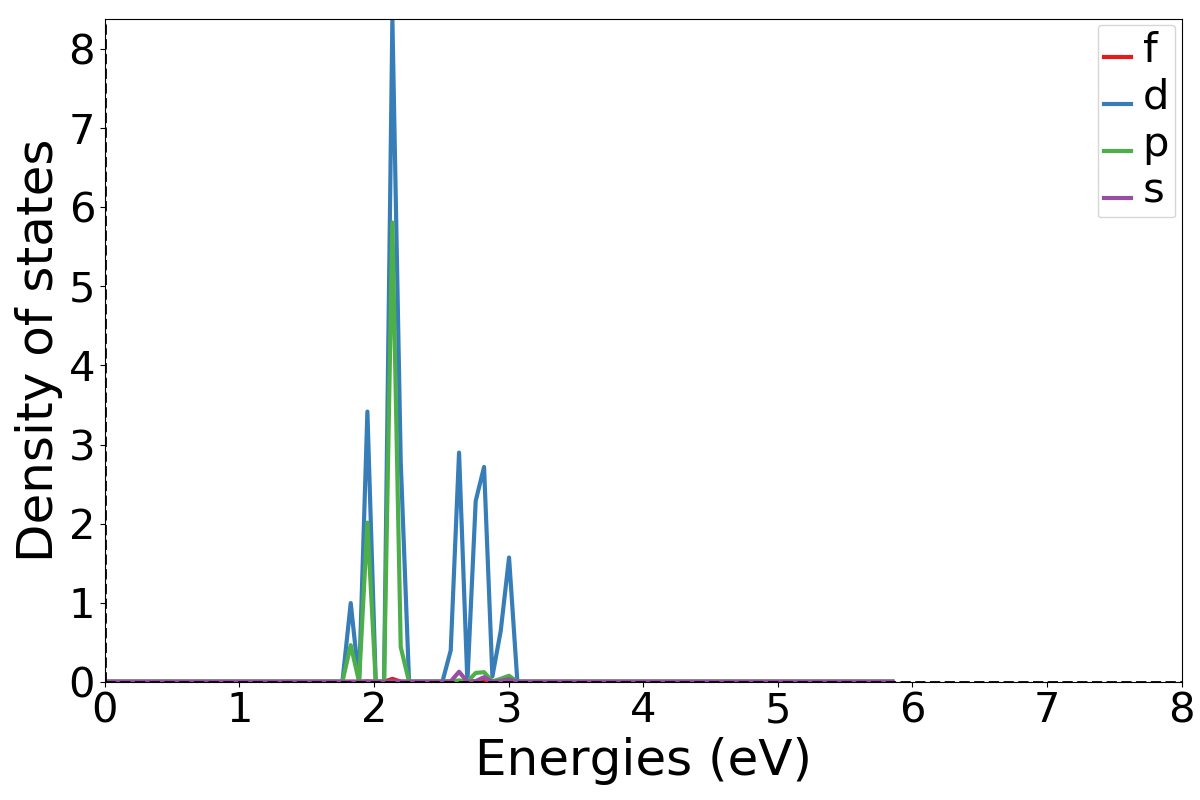
\includegraphics[width = 11cm]{../fig/Yb_k4_LDOS25_2.png}
      \caption{. }
      \label{fig:Yb_k4_LDOS25_2.png}
  \end{figure}

  \begin{figure}[H]
      \centering
      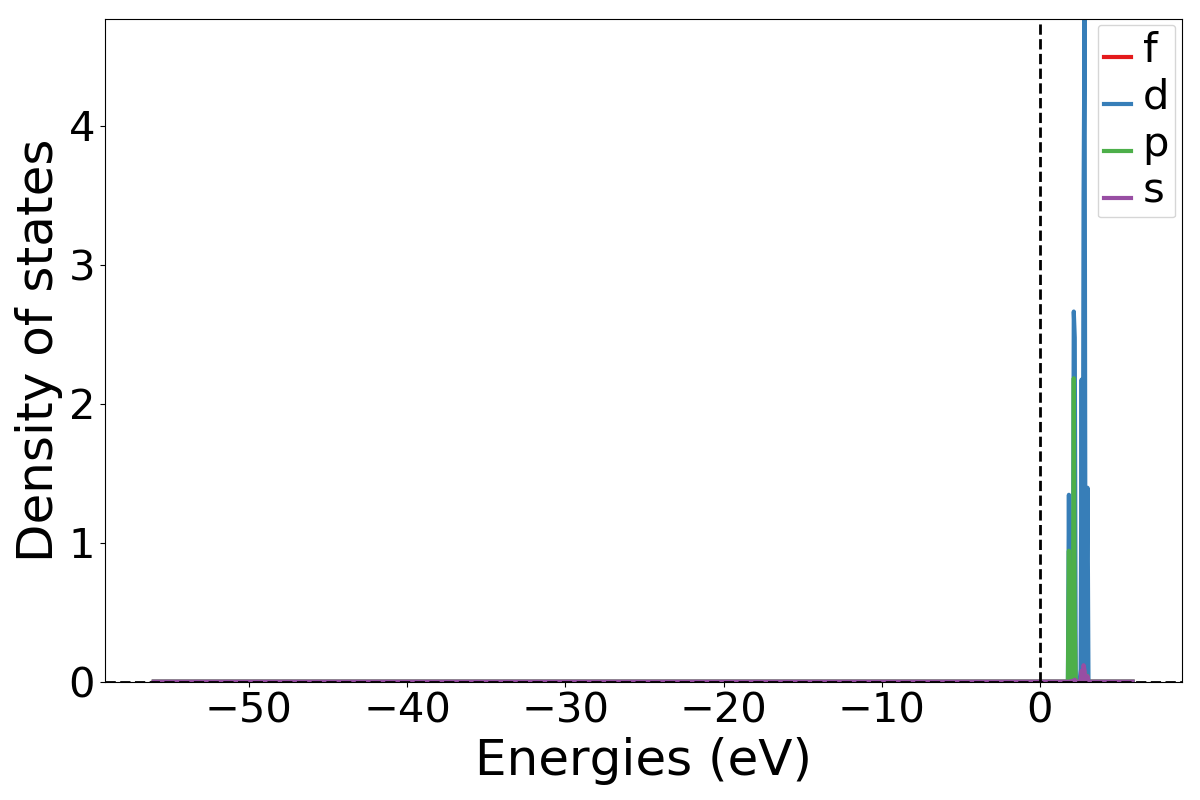
\includegraphics[width = 11cm]{../fig/Yb_k4_LDOS26_1.png}
      \caption{. }
      \label{fig:Yb_k4_LDOS26_1.png}
  \end{figure}

  \begin{figure}[H]
      \centering
      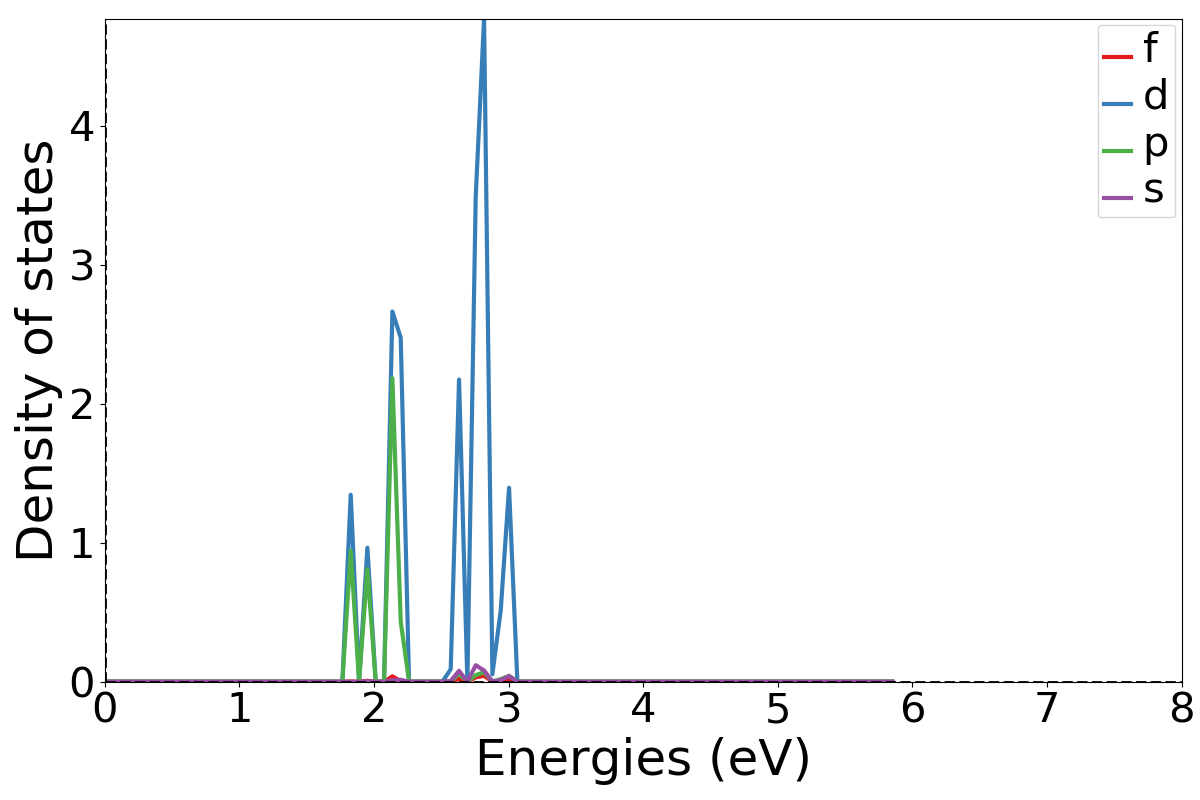
\includegraphics[width = 11cm]{../fig/Yb_k4_LDOS26_2.png}
      \caption{. }
      \label{fig:Yb_k4_LDOS26_2.png}
  \end{figure}

\vspace{1cm}

\section{Appendix 2}

    \iffalse
    \begin{python}
        import numpy as np

        N = 100

        x = np.linspace(1, 100, N)

        def f(x):
            return x**2

        y = f(x)

        print(y)


        test for cpp, men er nok bedre med den andre versjonen med lstlisting

        std::cout << "index, value\n";
      for(int i = 0; i < n; i++){
          std::cout << "    " << i << ", " << d_new[i] << std::endl;
      }

    \end{python}

    \begin{lstlisting}[language = python] — må huske å ha den ekstra delen til farger osv.
    \end{lstlisting}
    \fi

    \iffalse
    \begin{figure}[H]
        \centering
            \begin{tikzpicture}
            \draw[black, thick, ->] (-3,0) -- (4,0) node[anchor=west] {$x$};
            \draw[black, thick, ->] (0,-3) -- (0,3) node[anchor=south] {$\rho(x)$};
            \draw[cyan, thick, |-|, densely dashed] (-0.2,2.3) -- (3,2.3) ;
            \draw[cyan] (1.8,2.3) circle [radius = 0.01pt] node[anchor= south east] {$W$};
            \draw[thick] (0,0)--(0,2)--(3,2)--(3,0)--(0,0);
            \draw[text=cyan] (1,1.2)  node[anchor=north west] {$Q_s$};
            \fill[black] (3,0) circle [radius = 1.5pt] ;
            \draw[text=cyan] (3,0) node[anchor = north] {$x_{n0}$};
            \draw[thick] (0,0)--(0,-2)--(-0.2,-2)--(-0.2,0)--(0,0);
            \draw[text=cyan] (-1,-1)  node[anchor=north west] {$Q_m$};
            \fill[black] (-0.2,0) circle [radius = 1.5pt] ;
            \draw[text=cyan] (-0.2,0) node[anchor = south east] {$x_{p0}$};
        \end{tikzpicture}
        \caption{Ladningstetthet i deplesjonssonen for Schottkyovergangen.}
        \label{fig:schottkyladningstetthet}
    \end{figure}

    \begin{figure}[H]
        \centering
        \resizebox{17cm}{11cm}{
            \begin{tikzpicture}
                \draw [blue, thick, decoration={markings, mark=at position 0.750 with {\arrow{>}}}, postaction={decorate}] (3,0) arc(0:180:3);
                \draw [blue, thick, decoration={markings, mark=at position 0.250 with {\Huge \arrow{>}}}, postaction={decorate}] (3,0) arc(0:180:3);
                \draw [red, thick, decoration={markings, mark=at position 0.250 with {\arrow{<}}}, postaction={decorate}] (-1.10,0) arc(0:180:0.4cm);
                \draw [red, thick, decoration={markings, mark=at position 0.250 with {\arrow{<}}}, postaction={decorate}] (1.9,0) arc(0:180:0.4cm);
                \draw[text=blue] (0,3) node[anchor=north west] {$C_\rho$};
                \draw [->](-5,0) -- (5,0)  node[anchor=west] {$x$};
                \draw [->](0,-2) -- (0,5)  node[anchor=north east] {$y$};
                \fill[black] (3,0) circle [radius = 1.5pt] ;
                \draw [red, thick, decoration={markings, mark=at position 0.5 with {\arrow{>}}}, postaction={decorate}](-1.114,0) -- (1.114,0)  node[midway, anchor= south west] {$\gamma_\rho$};
                \draw [red, thick](-3,0) -- (-1.886,0);
                \draw [red, thick](3,0) -- (1.886,0);

                \fill[black] (3,0) circle [radius = 1.5pt] ;
                \draw[text=black] (3,0) node[anchor = north] {$1$};
                \fill[black] (-3,0) circle [radius = 1.5pt] ;
                \draw[text=black] (-3,0) node[anchor = north] {$-1$};
                \draw[black] (0,1.5) node[cross] {};
                \draw[text=black] (0,1.5) node[anchor = west] {$\frac{1}{2}i$};
                \draw[black] (-1.5,0) node[cross] {};
                \draw[text=black] (-1.5,0) node[anchor = north] {$-\frac{1}{2}$};
                \draw[black] (1.5,0) node[cross] {};
                \draw[text=black] (1.5,0) node[anchor = north] {$\frac{1}{2}$};
            \end{tikzpicture} }
        \caption{Konturen til integralet.}
        \label{fig:kontur}
    \end{figure}

    \begin{figure}[ht]
        \centering
        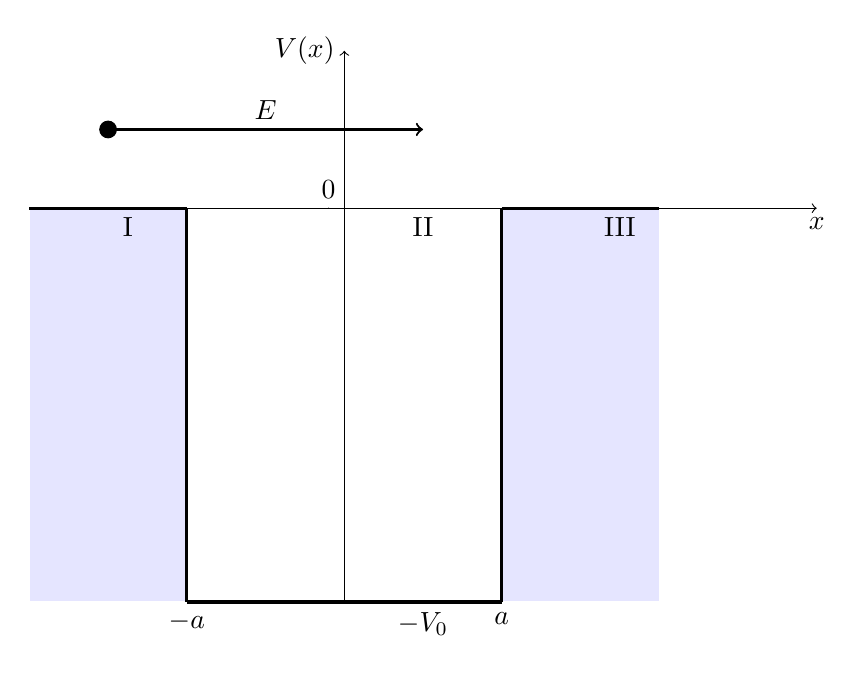
\begin{tikzpicture}
            \draw (-4,0) -- (-2,0);
            \draw (2,0) -- (4,0);
            \draw [fill = blue!10, draw = white] (-4,-5) rectangle(-2,0);
            \draw [fill = blue!10, draw = white] (2,-5) rectangle(4,0);
            \draw [->](0,-5) -- (0,2) node[anchor = east] {$V(x)$};
            \draw [->] (-4,0) -- (6,0) node[below] {$x$} node[very near start, below] {I} node[midway,below] {II} node[near end,below] {III};
            \draw[very thick] (-2,-5) -- (2,-5) node[near end, anchor = north] {$-V_0$};
            \draw[very thick] (-2,0) -- (-2,-5) node[below] {$-a$};
            \draw[very thick] (2,0) -- (2,-5) node[below] {$a$};
            \draw[very thick] (-4,0) -- (-2,0);
            \draw[very thick] (2,0) -- (4,0);
            \filldraw[black] (-3,1) circle(3pt);
            \draw[thick, ->] (-3,1) -- (1,1) node[midway,anchor = south] {$E$};
            \draw[very thin] (-0.2,0) circle(0.1pt) node[above] {0};
        \end{tikzpicture}
        \caption{Figur over potensialet for oppgave {\bf 4a)}.}
        \label{fig:4a}
    \end{figure}

    \begin{figure}[H]
        \centering
        %\resizebox{15cm}{17cm}{
            \begin{tikzpicture}
                \draw [->](-5,0) -- (5,0)  node[anchor=west] {$x$};
                \draw [->](0,-2) -- (0,4)  node[anchor=north east] {$y$};
                \fill[black] (0,0) circle [radius = 3pt] ;
                \fill[black] (3,0) circle [radius = 3pt] ;
                \draw[text=black] (3,0) node[anchor = north] {$-q$};
                \fill[black] (-3,0) circle [radius = 3pt] ;
                \draw[text=black] (-3,0) node[anchor = north] {$-q$};
                \draw[text=black] (0,0) node[anchor = north west] {$2q$};
                \draw[text=black] (3,0) node[anchor = south] {$(a,0,0)$};
                \draw[text=black] (-3,0) node[anchor = south] {$(-a,0,0)$};
            \end{tikzpicture} %}
        \caption{CO$_2$-molekyl i $xy$-planet. }
        \label{fig:elmag}
    \end{figure}

    \begin{figure}[H]
        \centering
        \includegraphics[width = 11cm]{bilder/L20um_mosfet_litografi2.png}
        \caption{ Diodestrømmen gitt som funksjon av spenningen over dioden. }
        \label{fig:mosfet-20um-litografi2}
    \end{figure}


    \begin{table}[ht]
        \centering
        \caption{Forventet og målt resistivitet for Schottkydiodene fra firepunktsmålingen.}
        \vspace{2mm}
        \label{tab:schottkyresistivitet}
        \begin{tabular}{|c|c|}
            \hline
            Forventet resistivitet $\rho$ [$\Omega$cm] & Målt resistivitet $\rho$ [$\Omega$cm]  \\
            \hline \hline
            1 - 10 & 6.975 \\
            \hline
        \end{tabular} \\
        \hspace{0pt}\\
    \end{table}
    \fi


%---------------- Slutten av dokumentet ---------------------------------------

%\end{multicols}

\end{document}
